\chapter{Review of Theory and Prior Work} \label{txt:background-chapter}
% Michael: I would suggest (not require) that some more examples like the apples and bananas would make it easier to follow for readers who are not so into this complex area

\section{Aerosols and their Impacts on Health and Climate Change} \label{txt:aerosols}

The Earth's atmosphere is an oxidising environment. When \textbf{reduced} gases and particles, i.e. compounds that have some excess loosely-bound electrons, are emitted into our atmosphere, they are \textbf{oxidised}. Oxidation occurs when \textbf{oxidising} agents, which are highly \textbf{electronegative} because they lack electrons and strongly pull other electrons towards themselves, `steal' electrons from reduced compounds. These now-oxidised compounds are then deposited back to the surface into the Earth's biosphere, geosphere, and hydrosphere.

For instance, reduced \textbf{Volatile Organic Compounds} (\textbf{VOCs}) are emitted into the atmosphere through biogenic and anthropogenic (human-caused) sources, such as the scent of trees, chemical solvents, and fossil- and bio-fuel combustion. In the atmosphere, these VOCs undergo a cascade of oxidising reactions in which highly electronegative agents such as oxygen add themselves to the VOC to steal some of its electrons. This cascade transforms the VOCs into semi-, low-, and extremely low-volatile organic compounds and eventually results in the production of mostly $\text{CO}$, $\text{CO}_2$ and water. Not all compounds finish their complete breakup by oxidation but are instead deposited out of the atmosphere early. Most VOCs are short-lived because of their short chemical lifetimes and high deposition rates and can thus usually only reach the troposphere, which spans from the surface to an average height of $13 \text{km}$ \cite[p.~14]{atmospheric-chemistry-1999}. The very potent greenhouse gas methane ($\text{CH}_4$) is an exception as it has a lifetime of around a decade, allowing it to reach beyond the troposphere into the stratosphere \cite{methane-hydrates-2017, atmospheric-chemistry-1999}. Important biogenic VOC emissions include methane, mostly from wetlands, and isoprene ($\text{C}_5\text{H}_8$) and monoterpenes ($\text{C}_{10}\text{H}_{16}$) such as $\alpha$-pinene and $\beta$-pinene, mainly from forests. Important anthropogenic emissions include carbon monoxide ($\text{CO}$), methane, sulfur dioxide ($\text{SO}_2$), ammonia ($\text{NO}_3$), and nitric (di-)oxide ($\text{NO}_{x}$). Please refer to \textcite{atmospheric-chemistry-1999} for a comprehensive introduction to atmospheric chemistry. % p.134
% Petri: It is good to remember that CO2 (and CO) is the final product only for some compounds. Many others just keep getting heavier. In some oxidising reactions, they might shed some light compound which turns to CO2 and water later, but often the large molecules get removed from the atmosphere before their complete breakup.

\newpar \textbf{Aerosols} are solid or liquid particles suspended in a gas such as air \cite[p.~144]{atmospheric-chemistry-1999}. They significantly affect our health and climate. Where do these particles, sized between $10^{-9}\text{m}$ to $10^{-4}\text{m}$, come from? They can be divided into primary and secondary aerosols\footnote{Cloud-phase-induced aerosols are similar to secondary aerosols but are produced inside an evaporating cloud droplet \cite{cloud-aerosol-1996}.}, where the former includes particles that are emitted directly, e.g. from natural emissions such as volcanic ash, dust, sea salt, and pollen. In contrast, secondary aerosols are formed from low-volatile and reactive atmospheric compounds like nitric or sulphuric acid. They undergo a formation process starting with the nucleation of tiny molecular clusters, which then grow through condensation and collisions with other particles (coagulation). Thus, aerosols are further divided by size into one coarse particle mode ($10^{-6}\text{m}$ -- $10^{-4}\text{m}$) and three fine particle modes: the nucleation mode ($10^{-9}\text{m}$ -- $10^{-8}\text{m}$), Aitken mode ($10^{-8}\text{m}$ -- $10^{-7}\text{m}$), and accumulation mode ($10^{-7}\text{m}$ -- $10^{-6}\text{m}$). \Cref{fig:aerosol-emission-effects} provides an overview of the diverse sources and effects of aerosols, which are discussed in more detail below.

Aerosol particles significantly impact our health. While our nose and throat catch most big particles, smaller ones can reach our lungs and even be absorbed into our bloodstream through the alveoli, from where they can reach our organs \cite{aerosol-airways-2005}. Thus, aerosols are particularly hazardous to human health if they are small and reactive. For example, in 2019, the last pre-pandemic year for which data is available, around 307,000 premature deaths in EU-27 countries were attributed to chronic exposure to fine particulate matter \cite{eu-health-2021}. In addition to respiratory problems, long-term pollution exposure can ``cause vascular and brain diseases'' \cite{aerosol-health-2020} and increase the risk for depression \cite{pm-depression-risk-2022}. Moreover, even short-term exposure is dangerous as it reduces visibility in highly polluted urban areas during smog events and increases the suicide risk among major depressive disorder patients \cite{pm-suicide-risk-2022}.

\begin{figure}[H]
    \centering
    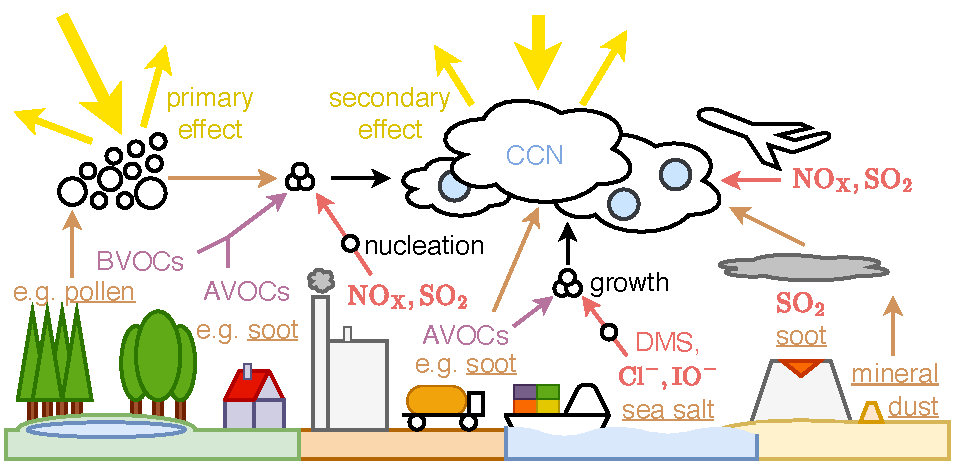
\includegraphics[width=0.9\textwidth]{background/figures/aerosols.pdf}
    \caption[Overview of the sources, formation process, and impacts of aerosols]{Overview of the sources, formation process, and impacts of aerosols. \textcolor{primary-aerosol}{\textbf{\underline{Primary aerosols}}} are emitted directly, while \textcolor{aerosol-precursor}{\textbf{precursors}} form \textbf{secondary aerosols} that can then grow with oxidised \textcolor{aerosol-voc}{\textbf{VOCs}} into \textcolor{aerosol-ccn}{\textbf{Cloud Condensation Nuclei}}. Note that $\approx 55\%$ of \textcolor{aerosol-ccn}{\textbf{CCN}} come from \textcolor{primary-aerosol}{\textbf{\underline{primary emissions}}} and $45\%$ from \textbf{secondary aerosols} \cite{ccn-sources-2009}. Aerosols have health, visibility, and \textcolor{aerosol-climate}{\textbf{primary and secondary climate effects}}.}
    \label{fig:aerosol-emission-effects}
\end{figure}

\noindent Aerosol particles also impact our climate. They have a direct radiative forcing effect on the energy balance of the atmosphere as they scatter (and absorb) light and thus mostly\footnote{Black carbon, on the other hand, is an aerosol that contributes to global warming \cite{ipcc-6-summary-2021}.} reduce some of the sun-driven warming of the Earth. Additionally, aerosols also impact the formation of clouds\footnote{While aerosols also impact cloud dynamics, these are out of scope for this summary.}. The (cloud) droplets that clouds consist of do not form from just water molecules alone, as the air is not saturated enough by water in the atmosphere to initiate homogeneous nucleation \cite{ccn-1999}. Instead, ice particles/nuclei (IN) or \textbf{Cloud Condensation Nuclei} (\textbf{CCN}), which are aerosols in the Aitken and accumulation modes, are needed so that the water vapour can deposit or condense on them and form ice crystals or cloud droplets, respectively. If more CCN and IN are produced, the water in the atmosphere is distributed across more nuclei on which it can condense. Thus, more but smaller cloud droplets are created, which in turn increases the lifetime of clouds and reduces the intensity of rain. Furthermore, clouds with more and smaller cloud droplets scatter more light and have a higher albedo and can thus better reflect light. Therefore, the overall net effect of aerosols is estimated to be cooling, even though some aerosol interactions, such as black carbon emissions, have warming effects \cite{ipcc-6-summary-2021}. However, the extent of this cooling effect is still unclear, and aerosols are the among the largest sources of uncertainty in the IPCC reports that aim to predict the extent of future global warming \cite{ipcc-6-summary-2021}.

\section{An Introduction to the SOSAA Model} \label{txt:sosaa-model}

Modelling atmospheric chemistry is essential to understand the impacts that anthropogenic emissions and our changing environment have on human health and climate change. Complex processes such as surface emission fluxes, turbulent transport, meteorology, aerosol formation, dry and wet deposition, and chemical reactions interact in the atmospheric boundary layer (ABL), which starts from the Earth's surface and can reach up to several kilometres \cite{sosa-description-2011}. However, many aspects of especially aerosol processes are still unknown and the subject of ongoing research. The complexity of simulating these interacting processes requires choosing between (a) simulating a small box volume for a short time at a high level of detail or (b) applying broad simplifications so that an approximate chemistry scheme can be simulated inside a global weather or climate simulation.

\newpar SOSAA, the model to \textbf{S}imulate \textbf{O}rganic vapours, \textbf{S}ulphuric \textbf{A}cid and \textbf{A}erosols, is a chemistry transport model that was originally implemented in \textcite{sosa-description-2011} ``to reconstruct the emissions, transport and chemistry in the ABL [atmospheric boundary layer]'' \cite{sosa-description-2011} around the Finnish measurement station SMEAR II at Hyyti\"al\"a \cite{smear-station-2013}. It models the atmospheric processes inside a one-dimensional height column, which starts from the Earth's surface and reaches up to a height of a few kilometres, using several box models stacked on top of each other. Each box simulates its internal processes independently for a given time step, after which turbulent mixing drives the chemical transport between the boxes and exchanges species concentrations. Then, the procedure is repeated for the next time step. Given the reduced 1D dimensionality of the model, SOSAA ignores both horizontal and vertical advection and thus works best in open, flat, and horizontally-homogeneous terrain, e.g. the boreal forest around Hyyti\"al\"a. \Cref{fig:sosaa-overview} shows the modules SOSAA consists of, which are implemented in Fortran and coupled by the meteorology that controls the chemical exchange.

\newpar Since its original implementation in \textcite{sosa-description-2011}, SOSAA has been continuously improved and applied in various studies, including \cite{sosaa-description-2014, sosaa-bvoc-2017, sosaa-ozone-2017, sosaa-trends-2021}. The simulation uses MPI, the Message Passing Interface, to parallelise the computation of the chemical kinetics and aerosol processes in different boxes. In contrast, the emissions, deposition, meteorology, and mixing of chemical species are serialised. SOSAA is highly customisable and supports changing the number and spacing of the height column of boxes (usually around $50$ boxes reach up to $3 \text{km}$), the time steps of different modules (usually the meteorology uses $\Delta t = 10 \text{s}$ while all other modules run at a lower frequency and $\Delta t = 60 \text{s}$), and toggling which atmospheric processes are included in the simulation.

\begin{multicols}{2}
    \begin{figure}[H]
        \centering
        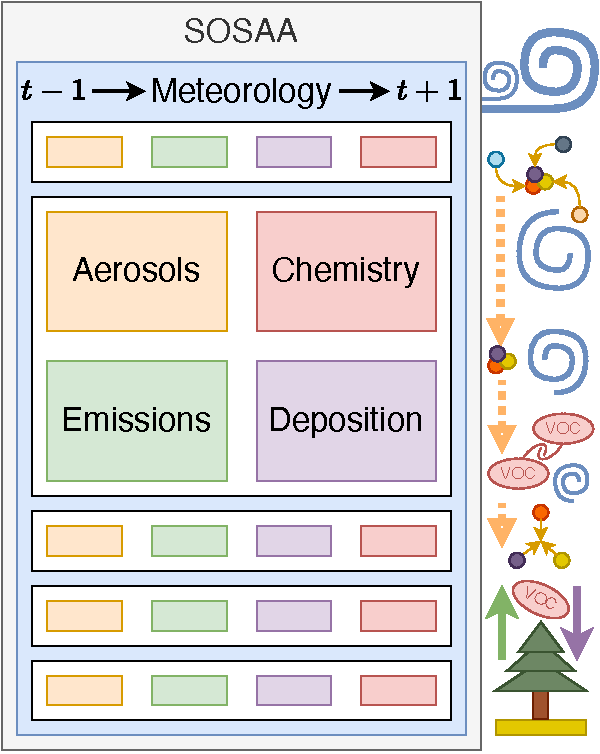
\includegraphics[width=0.49\textwidth]{background/figures/sosaa.pdf}
        \vspace{-1em}
        \caption[Overview of the Modules of the SOSAA Model]{Overview of the modules of the SOSAA model. SOSAA consists of a 1D stack of boxes that simulate emissions, deposition, chemical kinetics and aerosol processes. They are coupled through the meteorology.}
        \label{fig:sosaa-overview}
    \end{figure}

    \begin{enumerate}
        \item The \textbf{meteorology} module is a 1D version of the coupled plant-atmosphere boundary layer model SCADIS \cite{scandis-model-2002, scandis-analysis-2005, scandis-drag-2006}, which provides chemical mixing and transport between the thus-coupled boxes \cite{sosa-description-2011} and includes the ``prognostic equations for the horizontal wind vector, air temperature and absolute humidity'' \cite{sosaa-trends-2021}. In trajectory mode, global weather simulation outputs are used instead.
        \item The \textbf{emissions} module is a modified version of the MEGAN 2.04 \cite{megan-model-2006} model that provides plant canopy BVOC emissions, which are supplemented by governmental emission inventory data.
        \item SOSAA uses a chemistry reaction mechanism based on MCMv3.3.1 \cite{mcm-protocol-1997, mcm-v3-2003, mcm-beta-2012} for its \textbf{chemical kinetics}. The mechanism, which is compiled to Fortran using KPP \cite{kpp-preprocessor-2002}, simulates the time evolution of chemical species concentrations independently for each box model.
        \item Initially, the UHMA \cite{uhma-model-2004} model was used to simulate \textbf{aerosol} nucleation, condensation, coagulation and deposition processes. It is currently being replaced by the ARCA box model \cite{arca-box-2022}.
        \item \textcite{sosaa-bvoc-2017} added a multi-layer gas-\textbf{dry deposition} module \cite{gas-exchange-2002} to investigate the effect that not modelling the forest canopy as just one big leaf has on the atmosphere-biosphere gas-exchange and canopy gas-concentrations \cite{sosaa-bvoc-2017, sosaa-ozone-2017}.
    \end{enumerate}
\end{multicols}

\noindent The initial implementation of SOSAA only supported a stationary mode where the column of boxes remains in one location. In this mode, SOSAA models the atmospheric processes for a nearby measurement station like SMEAR II at Hyyti\"al\"a \cite{smear-station-2013}. Since high-quality measurement data are available at the station, SOSAA is continuously nudged towards the observations, which has allowed modelling the processes behind long-term trends in $\text{OH}$, $\text{NO}_3$ and $\text{H}_2\text{SO}_4$ concentrations at Hyyti\"al\"a \cite{sosaa-trends-2021}. More recently, a Lagrangian trajectory mode has been under development. In this mode, the trajectories of air parcels arriving at a measurement station are first calculated backwards in time, e.g. using FLEXPART \cite{flexpart-validation-1998, flexpart-correction-1999, flexpart-6.2-2005, flexpart-10.4-2019}. Next, the emissions and meteorological conditions along this trajectory are gathered from global weather models and emission databases. Finally, SOSAA is run along the trajectory by moving the box column to follow the path from the particle origins to the measurement station destination. Throughout, SOSAA is given the local meteorological conditions and the local aerosol, anthropogenic, and biogenic emissions. Whereas the stationary mode can use high-resolution and high-quality local measurement data, the trajectory mode often needs to interpolate more coarse data sources along the trajectory. Thus, the accuracy of some locally available variables is traded for new insights that the Lagrangian trajectory mode can give on far-away emission sources and the transport of aerosols and chemicals.

\newpar Unfortunately, the SOSAA model is not yet publicly available. However, access to the complete SOSAA source code is provided upon request -- please contact Michael Boy (\href{mailto:michael.boy@helsinki.fi}{michael.boy@helsinki.fi}), Putian Zhou (\href{mailto:putian.zhou@helsinki.fi}{putian.zhou@helsinki.fi}), or Petri Clusius (\href{mailto:petri.clusius@helsinki.fi}{petri.clusius@helsinki.fi}) for more information. All SOSAA model runs for this thesis were performed with \href{https://version.helsinki.fi/putian.zhou/sosaa/-/tree/10618aa98c7470546308adf132afb0bc0735b4eb}{SOSAA@10618aa}.

\section{A brief Introduction to Machine Learning} \label{txt:machine-learning}

Machine Learning is a field of research that investigates and develops methods that learn new behaviours by being shown examples of the behaviour and receiving feedback on their performance. More formally, \textcite{machine-learning-1997} gives the following definition:
\begin{center}
    ``A computer program is said to \textbf{learn} from experience $E$ with respect to some class of tasks $T$ and performance measure $P$ if its performance at tasks in $T$, as measured by $P$, improves with experience $E$.''
\end{center}
For instance, machine learning can train a smartphone camera to detect faces in an image. In this case, the \textbf{task} is to identify which rectangular areas in an image contain faces. To \textbf{train} the camera for this task, it is shown images that contain faces. The more images it is shown, the more \textbf{experience} the algorithm has with detecting them. Often it is also informed about the true locations of all faces in all images. Finally, the detection algorithm's \textbf{performance} is \textbf{evaluated} by calculating a punishment score, called the loss function $\mathcal{L}$, that increases the further away and differently sized each predicted face is from the actual face locations in each image.

\newpar Machine Learning is part of the broader academic discipline of Artificial Intelligence \cite{ai-review-2008}, which also encompasses fields such as genetic algorithm optimisations, logic-based reasoning, knowledge representation, and artificial life. Machine Learning combines ideas from data science, mathematical fields like statistics, as well as algorithms and computational methods from computer science. Insights from the natural sciences also often inspire progress in machine learning \cite{biological-dnn-2021}. Given this diversity of backgrounds in machine learning, it is imperative to define the terms, notations, and symbols that this thesis uses:
\begin{enumerate}
    \item \textbf{Variables} are represented with one letter, e.g. $X$ or $y$. Lowercase letters refer to vectors, while uppercase letters represent matrices. For instance, a dataset $X$ of face positions contains many rows $x$, each encoding example of a face. The columns of the dataset encode the face's features, e.g. its image location.
    \item A machine-learning \textbf{algorithm} or \textbf{method} refers to the description of how to construct, train, and evaluate a machine to learn a certain task. In contrast, a machine-learning \textbf{model} is an instance of a method. While a method is designed by a human, a model is trained by the machine to improve its performance on its given task. A model's tunable configuration options are called its trainable \textbf{parameters}, while the method's options are referred to as \textbf{hyperparameters}.
    \item In \textbf{supervised} Machine Learning, a model is trained by being given examples of both the \textbf{input} and \textbf{target output} for the specific task. In contrast, an \textbf{unsupervised} model is trained with only the inputs. The third machine learning paradigm is \textbf{reinforcement} learning, where the model actively explores the input space, decides which action to take, and is rewarded or punished according to its performance.
    \item Supervised models are trained with a \textbf{training} set $(X_{train}, Y_{train})$ that contains pairs of input-output examples $(x, y)$. The columns of the input are called \textbf{features}, while the rows are often called \textbf{samples}, \textbf{examples}, or \textbf{points}. Some methods use a separate \textbf{validation} set $(X_{valid}, Y_{valid})$ to further finetune a model after training. Finally, the model is tested on the inputs for a \textbf{test} set $X_{test}$. The model's predictions for the target output, denoted as $\hat{Y}$, are then compared to the \textbf{true} target outputs $Y_{test}$ to evaluate the model's performance. Thus, the goal of a supervised model is to learn the process $f(X) = Y$ behind the training data and approximate the outputs with its predictions $\hat{Y} \approx Y$.
    \item \textbf{Regression} models predict continuous outputs. In contrast, \textbf{classification} models learn to predict one (single-class) or more (multi-class) options from a fixed set of discrete output \textbf{classes}.
\end{enumerate}

\noindent This section provides a brief and targeted overview of a few machine learning methods. In particular, \Cref{txt:linear-model} introduces the Classical Linear Regression Model and the assumptions it is built upon. Next, \Cref{txt:data-preprocessing} highlights how the training data can be preprocessed to support the learning process. \Cref{txt:bootstrapping} and \Cref{txt:ensembles-decision-tree-random-forest} continue by introducing bootstrapping and ensemble methods, which are demonstrated with the example of decision trees and random forests. Following on, \Cref{txt:padre-rf} reviews the Pairwise Difference Regression method that is designed to make robust predictions even with little training data. Next, \Cref{txt:neural-network} provides the brief background on neural networks that this thesis requires, while \Cref{txt:auto-differentiation} dives deeper into the topic of automatic differentiation. Finally, \Cref{txt:ml-libraries} introduces the machine-learning libraries that are used in this thesis. Please refer to \textcite{machine-learning-1997} for a more comprehensive introduction to machine learning.

\subsection{The Classical Linear Regression Model} \label{txt:linear-model}

The classical linear regression model is one of the simplest machine learning models. It attempts to fit a linear relationship between a set of $k$ independent input variables $X_1, ..., X_k$ and the output variable $Y$ by tuning the model intercept or bias $b$ and the regression coefficients $a_1, ..., a_k$ \cite{clrm-assuptions-1971}:
\begin{equation}
    Y = \sum_{i=1}^{k}{(a_i X_i)} + b + \epsilon
\end{equation}
where $\epsilon$ is an added error term that represents the effect of unknown input variables or inherent randomness in the system. Note that the bis $b$ is often integrated into the regression coefficients by introducing a new constant input $X_0 = 1$. The classical linear regression model should only be used to fit a dataset if the following assumptions about the input and output variables hold \cite{clrm-assuptions-1971}:
\begin{enumerate}
    \item \textbf{Non-random Input Measurements:} The values of the input-variables $X_1, ..., X_k$ are constant or contain only negligible measurement error.
    \item \textbf{Linearity:} $Y$ is linearly related to the input variables $X_1, ..., X_k$.
    \item \textbf{Linearly Independent Inputs:} The input variables $X_1, ..., X_k$ are linearly independent, i.e. none can be expressed as a linear combination of the others.
    \item \textbf{Normal Error:} $\epsilon$ is normal distributed with zero mean.
    \item \textbf{IID Error:} $\epsilon$ is independently (no correlation between errors) and identically (the error distribution is constant across the input domain, i.e. homoscedastic) distributed.
\end{enumerate}

\noindent It is clear that at least $k+1$ input-output pairs are required to fit the parameters of this linear model. However, since the error term $\epsilon$ is often not zero, e.g. because of randomness or missing inputs, identifying the exact solution is not possible in general. In that case, the ordinary least-squares solution that minimises the squared error $(y_i-\hat{y}_i)^2$ can be found for $N$ input-output pairs $(x_i, y_i)$ \cite[P/mlr-ols]{stats-proofs-2022}:
\begin{equation}
    \begin{split}
        \hat{b} &= \argmin_{b}{\sum_{i=1}{N}{\left( b \cdot x_i - y_i \right)^2}} \\
                &= {\left( X^{\intercal} X \right)}^{-1} X^{\intercal} Y
    \end{split}
\end{equation}
To avoid overfitting on noisy samples, it is recommended to fit the model on more than the required $k+1$ input-output pair training samples.

\subsection{Preprocessing Data for Effective Machine-Learning} \label{txt:data-preprocessing}

Many machine-learning algorithms are not `off-the-shelf' but require hyperparameter tuning of the method or preprocessing of the dataset \cite{statistical-learning-2009} to perform well\footnote{Random forests (see \Cref{txt:ensembles-decision-tree-random-forest}) require little tuning and are thus one notable exception \cite{ml-hyperparameters-2021}.}. This subsection provides a very brief overview of different data preprocessing methods to improve a model's training process. Please refer to \textcite{data-preprocessing-2007} for a more extensive introduction to data preprocessing for supervised learning.

\newpar Input data can be of different kinds, including continuous and discrete quantitative features, or nominal and ordinal qualitative data \cite{feature-selection-2014}. However, when a given model does not support all of these datatypes, it is necessary to convert between them. For instance, ordinal features such as letter grades from \texttt{A} to \texttt{F} can be transformed into discrete integers or the continuous test score percentages associated with these marks. For nominal features, where no order of the set of inputs exists, the one-hot encoding transforms each value into a binary feature that indicates whether or not the specific value is present. Continuous inputs can also be discretised into a reduced range of statically or dynamically selected bins \cite{data-preprocessing-2007}.

The collected training dataset may also contain errors such as missing values and outliers with unexpectedly high measurement errors. Some methods, such as decision trees, can explicitly deal with missing values \cite{machine-learning-1997} and are robust to outliers \cite{statistical-learning-2009}. For other methods, however, it may be necessary to filter out outliers using novelty detection (see \Cref{txt:novelty-detection}) and replace missing values with the feature mean, mode, or the value that is most often observed with similar inputs \cite{data-preprocessing-2007}.

ML models learn through the evaluation of their performance on a training dataset. If they are trained on a skewed dataset that does not reflect the true input distribution, they often overfit on the skewed data and thus perform worse on minority inputs \cite{ml-bias-discrimination-2017}. In such cases, either stratified sampling or data reweighting should be used \cite{data-preprocessing-2007}. While stratified sampling finds a training subset in which the different outcomes are represented equally, reweighting gives minority samples higher weight such that all samples are used, and the model is forced to be more careful with minority inputs even though they are still underrepresented in the training data.

\newpar ML models are generally constructed for fixed-size inputs and outputs. However, input domains such as images can be of arbitrary sizes, and tasks such as detecting the locations of all faces in an image may require variable-sized output lengths. Fixed-sized models can be trained and applied to this data by only providing them with a fixed-size window view of the data that is shifted across the input and for which they then make a fixed-size prediction. To account for variations in scale, a pyramid of several increasingly large, typically increasingly downsampled windows can also be provided as input \cite{feature-pyramid-1984}.

Training a model on a high-dimensional dataset is often challenging as computational performance decreases with increasing dimensionality \cite{ml-pattern-2006}, noise increases, and the distances between inputs become more difficult to interpret. Therefore, reducing the input dimensionality is often beneficial and acts as a feature selector to remove redundant or unimportant features. Principal Component Analysis (PCA) is among the most popular linear dimensionality reduction methods. PCA identifies a new set of orthogonal basis vectors, the principal components, that best explain the variance in the data. In particular, if $k$ principal components have already been identified, the $k+1$ component is the one that explains most of the still unexplained variance \cite{pca-1901}. Thus, projecting the data onto the $k$ first principal components produces the $L_2$-norm-optimal linear dimensionality reduction into $k$ dimensions. Note that PCA can also be extended to non-linear dimensionality reduction, e.g. by first applying a non-linear transformation kernel to the data \cite{kernel-pca-1997}.

PCA is very sensitive to the scale of the input variables, which becomes problematic if different features have different units and scales. It is thus recommended to first standardise the input by subtracting each feature's mean and rescaling them to unit variance using $x' = (x - \text{E}[x]) \mathbin{/} \sqrt{\text{var}[x]}$. Standardising features is not only helpful with PCA but also with many other methods. For example, many algorithms use regularisation as a method against overfitting \cite{statistical-learning-2009}, which often discourages learning large model coefficients. However, if different features are of very different scales, such large coefficients may be required to explain the data, and regularisation may thus make the learning process unnecessarily slow \cite{data-preprocessing-2007}. Normalising features using $x' = \frac{x - \min(x)}{\max(x) - \min(x)}$ is an alternative approach to transform all features to comparable ranges. If the inputs span several orders of magnitudes, it may be beneficial to first take the logarithm of the inputs before rescaling them. Alternatively, the cumulative distribution of the inputs can be approximated to transform the inputs into a percentile score.

In addition to feature selection, new features can also be constructed. For instance, polynomial expansion and non-linear transformations can be applied to the features of a linear regression model (see \Cref{txt:linear-model}) to allow it to fit non-linear processes. It is also often possible to manually construct new features using domain-specific background knowledge.

\newpar While this subsection has only given a brief overview of feature preprocessing, it still highlights the expansive scope of this topic and the available options. AutoML Methods such as Auto-WEKA \cite{automl-2013} or Auto-sklearn \cite{auto-sklearn-2019} have thus been developed to reduce the need for manual configuration of the entire data preprocessing pipeline.

\subsection{Estimating Errors with Bootstrapping} \label{txt:bootstrapping}

Machine Learning has increased in accessibility, performance, and popularity with the increase in big data and highly parallel compute performance \cite{ml-trends-2021}. Today, many machine learning methods require large datasets to train a model, and high-confidence analysis of their performance requires collecting statistics over large data samples. However, such large amounts of data are only sometimes available. Therefore, squeezing as much information as possible out of smaller datasets is beneficial.

\newpar \textcite{bootstrapping-1979} introduced the Bootstrapping method to compute any statistic for an unknown distribution using only a small independently and identically distributed (iid) sample from the population. In its most basic form, resampling with replacement is used to generate $M$ different resamples of size $N$ for the original dataset of size $N$. Next, the target statistic is calculated independently for each of the $M$ resamples. Finally, the $M$ different results are combined, and their distribution is reported. Even though only data from the original small sample is used, bootstrapping can estimate the population statistic with much higher quality than only calculating the statistic on the original sample would have achieved.

For example, say we have a small set of noisy ozone concentration measurements from an urban area. If we are only interested in the sample mean, we can simply average all measurement samples. However, in this case, we want to estimate the population mean and its confidence interval. Therefore, we generate $M$ new synthetic datasets by resampling the measurements with replacement, i.e. some measurements are included multiple times in one synthetic dataset, while others are excluded. Next, we calculate the mean for each of these resamples and thus produce a distribution of all the calculated means. We can now look at the cumulative distribution of the means to extract the $15.9\%$ and $84.1\%$ quantiles for the $1\sigma$ error and calculate the population mean as the mean of all means $\{\hat{\mu}\}_{i}$. In this example, the final reported result $\hat{\mu}'$ is
\begin{equation*}
    \hat{\mu}' = {\text{E}[\hat{\mu}]}^{+(\hat{\mu}_{84.1\%} - \text{E}[\hat{\mu}])}_{-(\text{E}[\hat{\mu}] - \hat{\mu}_{15.9\%})} 
\end{equation*}
\noindent Consider another example where we have a set of points that appear to have been generated by a simple process and some noise, e.g. $f(x) = a \cdot x + b + \epsilon$. While simply fitting a linear regression model to this data sample can give us the sample estimate for the gradient $a$ and intercept $b$, we are again interested in estimating these parameters and their uncertainties for the larger population that the samples originate from. While simply resampling the set of points is possible, we can do even better using our assumption that a linear regression model explains our data well. In particular, we can fit the model on the original sample and record the error residuals between the predicted line and the samples. Next, we apply bootstrapping on the set of residuals to resample them, add them back onto the fitted line, and generate completely new sets of points. Finally, a regression model can be fitted to each of these datasets to find their $a$s and $b$s, which can then be reported as described above using both their mean and $1\sigma$ confidence interval.

\newpar Bootstrapping is not only limited to simple statistics, however. For example, when a neural network (see \Cref{txt:neural-network}) is trained, it is often optimised on the same data several times. To capture as much information from the original training data as possible, bootstrapping can be used to resample the training data on every training epoch. The same approach is also used when networks are optimised on smaller subsampled batches instead of the whole dataset, which can be computationally more efficient. Last but not least, bootstrapping can also help with training several instances of the same model on resamplings of the original training data. These resamplings can then provide an ensemble of slightly different predictions, which is covered in \Cref{txt:ensembles-decision-tree-random-forest}.

\subsection{Ensembles: from Decision Trees to Random Forests} \label{txt:ensembles-decision-tree-random-forest}

How can one tell apart apples, bananas, and oranges? Apples are often red, bananas are usually yellow, and oranges are generally orange. However, apples and bananas can also both be green, some apples are yellow, bananas turn brown, and red bananas and oranges both exist. What about their shapes? While apples and oranges are both round, bananas are distinctly crescent-shaped. By looking at the shape first, bananas can thus be distinguished. Amongst the round fruit, orange ones can be classified as oranges. However, further details, such as texture, would be needed to distinguish green, yellow, or red oranges from apples.

\newpar The development of such a hierarchical set of rules is also found in \textbf{decision trees}. Decision Trees are tree structures that make predictions on inputs by recursively traversing the tree structure from the root down to each input's associated leaf. At every node, an attribute of the input is checked to determine to which of the node's children the input belongs to. Decision Trees can most easily be applied to discrete input and output values \cite{machine-learning-1997}, e.g. the name of a fruit's colour and what type of fruit it is. Each leaf in a decision tree contains one or more training examples, which are combined to form a final prediction. For instance, the leaves in the fruit classification example above may use a majority vote to determine which fruit is most common in the round-and-orange leaf. Decision Trees can also be extended to continuous inputs and outputs. In this case, the leaf's prediction usually is the mean value amongst all training examples in this leaf.

The ID3 algorithm by \textcite{decision-trees-1986} is a fundamental algorithm to train a decision tree on a dataset with discrete-valued attributes. It is a greedy recursive algorithm that starts at the tree root with the full dataset $D$ and then repeatedly asks which attribute $A$ the data should be partitioned on to achieve the greatest information gain, i.e. the greatest reduction in entropy \cite{decision-trees-1986, machine-learning-1997}:
\begin{equation*}
    \begin{split}
        \text{Gain}(D, A) = \text{Entropy}(D) - \sum_{v \in \{ x_A \given (x, y) \in D \}}{\frac{|S_v|}{|S|} \cdot \text{Entropy}(D_v)} \quad &\text{where} \quad D_v = \{ (x, y) \given (x, y) \in D \land x_A = v \} \\
        \text{Entropy}(D) = \sum_{c \in \{ y \given (x, y) \in D \}}{\left( -p_c \cdot \log_{2}{p_c} \right)} \quad &\text{where} \quad p_c = \frac{|D_{y = c}|}{|D|}
    \end{split}
\end{equation*}
Once the split with the highest information gain has been identified, child nodes are added for each discrete attribute value, the dataset is partitioned into these nodes accordingly, and the procedure is repeated recursively on the child nodes. Note that information gain is only one of a range of possible split ranking functions. For instance, the gain ratio penalises splitting attributes that have many uniformly distributed values and which might thus seem like very distinctive features but may cause the decision tree to overfit \cite{decision-trees-1986, machine-learning-1997}:
\begin{equation*}
    \begin{split}
        \text{GainRatio}(D, A) &= \frac{\text{Gain}(D, A)}{\text{SplitInformation}(D, A)} \\
        \text{SplitInformation}(D, A) &= \sum_{v \in \{ x_A \given (x, y) \in D \}}{\left( -p_v \cdot \log_{2}{p_v} \right)} \quad \text{where } p_v = \frac{|D_{x = v}|}{|D|}
    \end{split}
\end{equation*}
where $\text{SplitInformation}(D, A)$ is the entropy of $D$ with respect to the values of the attribute $A$. To avoid selecting split attributes only because they mostly have the same value and thus low split information and a high gain ratio, \textcite{decision-trees-1986} suggest only choosing by the gain ratio on attributes with above-average information gain.

If all inputs are discrete-valued, an attribute that has already been used to split the dataset does not need to be considered for splitting in any descendent nodes. Continuous attributes can also be supported by dynamically identifying partitioning points that translate a continuous attribute $x$ into discrete attributes such as $x \leq 4.2$ and $x > 4.2$. Please refer to \textcite{continuous-tree-1992} for an introduction to how the optimal real-valued attribute threshold points can be found by testing a range of cleverly chosen thresholds.

\newpar While decision trees are highly capable and can ``represent any discrete-valued function defined over discrete-valued instances'' \cite[p.~76]{machine-learning-1997}, they can also suffer from overfitting on the training data. Even though trees can be pruned after training to improve their generalisability, constructing an entire forest with many trees is a much simpler approach. Random Forests, which were first introduced by \textcite{random-forests-1995}, use bootstrapping (see \Cref{txt:bootstrapping}) to train several independent decision trees on bootstrapped random resamples of the training dataset. Furthermore, bootstrapping is also applied to the attribute split selection, where only a random sample of the attributes is considered to greedily select the next split. In particular, \textcite{statistical-learning-2009} note that it is recommended to consider $\sqrt{F}$ of the $F$ features for classification problems and to have at least one example per leaf node, while only looking at $\frac{F}{3}$ features and requiring at least five examples per leaf for regression tasks. At prediction time, each decision tree makes an independent prediction, which are then aggregated using voting for classification and the mean for regression. Combining bootstrapping the dataset and its features and aggregating prediction results makes random forests more robust against overfitting than individual decision trees \cite{random-forests-1995}, even when the forest's hyperparameters are not explicitly tuned \cite{ml-hyperparameters-2021}.

\newpar Random Forests are an example of an ensemble method that trains a group of sub-models and then aggregates their predictions to improve their performance \cite{statistical-learning-2009, ensemble-learning-2020}. \textcite{ml-ensembles-2000} has identified ``the three fundamental reasons why ensemble methods are able to out-perform any single [model] within the ensemble'' \cite[p.~13]{ml-ensembles-2000}. First, if many different models can explain ambiguous observations equally well, combining them reduces the risk of choosing the single model that generalises the worst on unseen data. Second, each model may individually get stuck in a local optimum during optimisation. However, the combination of all submodels can escape some local minima and get closer to the global optimum. Third, while each method may not have sufficient complexity to represent the modelled process by itself, the model ensemble can represent more complex processes.

There are three main methods for constructing ensembles. Bootstrap aggregation (see \Cref{txt:bootstrapping}), also called \textbf{bagging}, uses bootstrapping to resample the dataset and train independent model instances of the same method on each of the resamples, whose predictions are then combined using voting or averaging. Bagging helps to reduce the variance of its submodels and can thus be used to avoid overfitting \cite{ensemble-overfitting-1995}. \textbf{Boosting} instead tries to reduce the bias of the ensemble by training the submodels sequentially. Each new submodel focuses on areas of the input domain where the already-trained models do not yet perform well \cite{statistical-learning-2009}. The combined prediction is then calculated as a weighted average over the submodel predictions. Since boosting ensembles have dependent members, boosting should only be applied when the base models already have low variance and are not prone to overfitting. Last but not least, \textbf{stacking} combines submodels that use different machine-learning methods. In addition to the submodels, a metamodel is trained that makes the final prediction based on each submodel's prediction. Stacking is thus closely related to model selection, but instead of only identifying which submodel performs best, it finds their optimal combination, thus leading to better predictions \cite{statistical-learning-2009}.

\subsection{Pairwise Difference Regression for Low-Data Tasks in Science} \label{txt:padre-rf}

How can a machine learning model generalise over a vast and complex feature space when only a few training examples are available? Augmenting the training data set is often used in tasks like image recognition or object tracking. For instance, an image can be cropped, rotated, scaled, or slightly damaged with noise without changing the target value that should be predicted. However, how can augmentation be achieved in scientific regression tasks, where cheaply inventing new data points with correct targets may not be possible?

\newpar \textcite{padre-rf-2021} present the \textbf{PA}irwise \textbf{D}ifference \textbf{RE}gression method PADRE, which builds on prior work by \textcite{pairwise-images-2018} of pairing training samples for augmentation. \citeauthor{padre-rf-2021} are motivated by predicting chemical properties such as a molecule's free energy, which are usually determined through \textit{very} computationally expensive yet approximate simulations. Since any single simulation has an unquantifiable error, several simulations are performed instead to calculate the difference between a new molecule and several known ones. Crucially, combining their different predictions somewhat cancels their errors. Inspired by this method from computational chemistry, the authors suggest training a model on the \textbf{differences} between molecules. In particular, given the training data set $\{ (X, Y)_1, (X, Y)_2, ... \}$, the model is now trained to predict the difference in output given a pair of inputs and their difference, i.e. $f(X_i, X_j, X_i - X_j) = Y_i - Y_j$ instead of $f(X_i) = Y_i$. Suppose the model is trained with all possible input pairs. Then, the number of training examples increases from $N$ to $N^2$, though it is worth noting that they still hold less information than $N^2$ ``normal'' independently and identically distributed (iid) samples. Nevertheless, the increase in inputs makes it more difficult for a machine-learning model to overfit on the small training dataset. At test time, an unseen data point $X_k$ is paired with every training point $(X_i, Y_i)$ to produce the final prediction $Y_k$:
\begin{equation*}
    Y_k = \frac{1}{N} \cdot \sum_{i=1}^{N}{\left(f(X_k, X_i, X_k - X_i) + Y_i \right)}
\end{equation*}
Unfortunately, training and testing on all input pairs also decrease the method's performance by a factor of $N$. Instead, a fixed-size random subsample of training points can be used (see \Cref{txt:bootstrapping}). Also, note that the pairwise input vector $X_i \bigoplus X_j \bigoplus (X_i - X_j)$, as chosen by the authors, is just one possibility. Another option, only using the difference between inputs, $X_i - X_j$, reduces the number of features but assumes that the output gradient is constant across the entire input space. In contrast, the matrix product $X_i \times X_{j}^{\text{T}}$ of both inputs includes the most information at the cost of a quadratic increase in features.

\newpar \citeauthor{padre-rf-2021} use Random Forests (see \Cref{txt:ensembles-decision-tree-random-forest}) as the base model for their PADRE-RF method since Random Forests are efficient to train, more robust to hyperparameter selection than Neural Networks \cite{ml-hyperparameters-2021}, and more robust to high-dimensional feature vectors than Gaussian Processes \cite{gp-dimensionality-2005}. The authors demonstrate that PADRE-RF outperforms a direct RF model on several datasets. They also utilise the spread of the predictions for each data point to measure the prediction uncertainty, which \citeauthor{padre-rf-2021} show to be correlated with the prediction error. The authors then utilise this uncertainty prediction to apply PADRE-RF in an active learning loop and select new training data that has high uncertainty under the current model.

\subsection{A Very Brief Introduction to Simple Neural Networks} \label{txt:neural-network}

(Artificial) Neural Networks are a biologically-inspired statistical machine learning method to approximate highly complex and non-linear functions. Neural Networks (NNs) are loosely inspired by our brains, where roughly one hundred billion neurons \cite{machine-learning-1997} communicate in a densely interconnected network of synapses. NNs attempt to replicate a simplified version of our natural neurons with artificial \textbf{neurons}, which are functions that take in signals from a range of input neurons and transform them into a single output signal that is used as input for other neurons. NNs are generally organised in layers, starting from the \textbf{input layer}, passing through an arbitrary number of internal \textbf{hidden layers}, to one or more \textbf{output layer}s. In each layer $l > 0$, $M_l$ denotes the number of neurons or units that are stacked in parallel. In a fully connected layer, all neurons take the outputs of all neurons in the prior layer $l-1$ as inputs. Each neuron can then be expressed as calculating the weighted sum over its inputs and applying a non-linear activation function $\phi(x)$ to the results \cite{rio-2019}:
\begin{equation*}
    z_{l, j} = \phi \left( \sum_{k=1}^{M_{l-1}}{w_{l,j,k} \cdot z_{l-1,k} + b_{l,j}} \right)
\end{equation*}
where $z_{l, j}$ is the output of the $j$\textsuperscript{th} neuron in the $l$\textsuperscript{th} layer, $w_{l,j,k}$ is the weighting factor for the input from the $k$\textsuperscript{th} neuron in the previous layer, and $b_{l,j}$ is a bias term for the weighted sum, which is often combined with the weighting factors by adding an extra constant one input to each layer. Note that $z_{0, j}$ represents the $j$\textsuperscript{th} feature of the input $x_j$ to the neural network and that $M_0$ is the input's dimensionality. To obtain a prediction, the neural network is evaluated in a layer-by-layer forward pass that eventually calculates the prediction as a non-linear activation of a weighted sum of the outputs of the penultimate layer. The network is fit to perform a specific task by optimising the weighting parameters of all neurons in the network.

\noindent Why should all hidden layers in a neural network use non-linear activation functions? While a linear activation function can be helpful to predict a real-valued output in a regression problem, a network with only linear activations effectively collapses into a single-layer neural network since ``the composition of successive linear transformations is itself a linear transformation'' \cite[p.~229]{ml-pattern-2006}. However, stacking many non-linear layers is what gives neural networks their capability to fit complex and non-linear processes since the network can build up increasingly higher-order features with each layer. For instance, multi-layer perceptrons are the simplest form of neural networks, consisting of three or more layers (including the input and output layers), all of which are fully connected. While MLPs were originally only built with perceptron units, some other simple but widespread activation functions that can also be used include \cite{activation-functions-2020, machine-learning-1997}:
\begin{enumerate}
    \item \textbf{Perceptron:} The sign function $\phi(x) = \text{sign}(x)$ is used to construct the perceptron unit, used in one of the oldest neural network architectures \cite{perceptron-1943}.
    \item \textbf{ReLU}: The rectified linear unit $\phi(x) = \max(0, x)$ is a cheap activation function with derivative $\phi'(x) = \max(0, \text{sign}(x))$ that produces sparse networks where some neurons are turned off for some inputs.
    \item \textbf{Sigmoid}: The sigmoid function $\phi(x) = \frac{1}{1 + e^{-x}}$ maps unbounded inputs to the $[0; 1]$ range and is thus often used in the final layer to produce binary classification probabilities. Its derivative is $\phi'(x) = \phi(x) \cdot (1 - \phi(x))$.
    \item \textbf{TanH}: The hyperbolic tangent function can be expressed by scaling and shifting the sigmoid function: $2 \phi(x) - 1$. It maps unbounded inputs to the $[-1; 1]$ range and can thus be conveniently used in hidden layers to describe the propagation of negative and positive activations.
\end{enumerate}
\noindent How are neural networks fit to learn a task? As noted by \textcite{machine-learning-1997}, machine learning for a specific task requires a performance measure with which the network can be evaluated on a set of training data. In supervised machine learning, the performance measure is often defined through a loss function $\mathcal{L}(y, \hat{y})$ which compares the expected true output $y$ with the prediction $\hat{y}$ and assigns a penalty for mistakes. The network is then trained to minimise this loss function for its predictions $\hat{y} = m(x)$. In regression problems, two common loss functions are the mean squared error loss $\mathcal{L}_{MSE}$ and the mean absolute error loss $\mathcal{L}_{MAE}$ \cite{ml-pattern-2006, mae-rmse-2005}:
\begin{equation*}
    \mathcal{L}_{MSE} = -\frac{1}{|D_{train}|} \sum_{(x, y) \in D_{train}}{(y - m(x))^2} \quad \quad \quad \quad \quad \mathcal{L}_{MAE} = -\frac{1}{|D_{train}|} \sum_{(x, y) \in D_{train}}{|y - m(x)|}
\end{equation*}
In binary classification problems, where the true label $y$ is either $0$ or $1$, the binary cross entropy loss $\mathcal{L}_{BCE}$ is minimised instead \cite{statistical-learning-2009}:
\begin{equation*}
    \mathcal{L}_{BCE} = -\frac{1}{|D_{train}|} \sum_{(x, y) \in D_{train}}{y \cdot \log(f(x)) + (1-y) \cdot \log(1-f(x))}
\end{equation*}
\noindent How can the network's parameters be optimised given a training dataset $D_{train}$ and the loss penalty that the neural network incurs for its (mis-)predictions? The gradient descent algorithm takes the gradient of the loss function with respect to all network parameters $w$ to find the change in parameters $\Delta w$ that produces the greatest reduction in the loss function. Once these per-parameter gradients are known, the weight parameters can be updated using $w := w - \eta \frac{\partial \mathcal{L}}{\partial w}$, where $\eta$ is a learning rate. The gradients are often averaged over a small random batch of samples or the entire training dataset to reduce their noise. This weight update is performed once for each training epoch, each of which represents one pass over the entire training data \cite{statistical-learning-2009}. If a neural network with sufficient capacity is trained long enough, it may start to `learn' the noise inherent in the training data sample and thus overfit. While regularisation methods attempt to limit how much detail the network can learn, encouraging it to prioritise underlying processes over noise, monitoring the prediction error on a validation dataset and stopping the training early when it no longer improves is another approach \cite{machine-learning-1997, statistical-learning-2009}.

Note that if the loss function is visualised as a landscape, the gradient descent algorithm continuously takes steps in the direction in which the landscape descends most steeply. However, if the optimisation starts in a depression surrounded by mountains, gradient descent is only able to find a local minimum, a common issue with complex non-convex learning problems. Therefore, more complex algorithms for updating the parameters and avoiding overfitting have been developed \cite{gradient-descent-overview-2017}.

\newpar How can the gradients of the loss function with respect to each of the network parameters be calculated efficiently? Using the chain rule of differentiation, $\frac{dy}{dx} = \frac{dy}{du} \cdot \frac{du}{dx}$, the gradient of the loss function can be decomposed into its gradient with respect to an output from the penultimate layer, and that output's gradient with respect to the parameter. While the first gradient can be derived from the definition of the current layer and its activation function, the second one can again be decomposed, leading to a repeated application of the chain rule. Thus, while inputs are propagated forwards through the network to make a prediction, loss gradients are propagated backwards from the output to the parameters in order to train the network. It is worth noting that the gradients of a neural network cannot only be used to optimise it. For instance, some adversarial methods use gradient descent to find the smallest change in the input that has the most negative impact on the prediction loss. The fast gradient sign method (FGSM), for example, constructs a small perturbation to an input $x$, e.g. the pixels of an image, to cause maximal misprediction \cite{fast-gradient-2014}:
\begin{equation*}
    x' = x + \epsilon \cdot \text{sign} \left( \frac{\partial \mathcal{L}(x)}{\partial x} \right)
\end{equation*}

\noindent This subsection has provided a very brief and basic introduction to neural networks. However, it entirely skips more advanced network architectures such as increasingly deep \cite{deep-learning-2019}, recurrent \cite{recurrent-nns-2019} or convolutional neural networks \cite{cnn-1990, cnn-review-2022}. Thus, please refer to the provided citations for an overview of recent advances in neural networks. Following on, \Cref{txt:auto-differentiation} delves into how the derivatives used in optimising neural networks can be derived automatically directly from the code that describes the forward prediction pass through the network.

\subsection{The Power and Promise of Auto-differentiation} \label{txt:auto-differentiation}

Neural networks are generally fit by using gradient descent to update their parameters to minimise a loss function. How are these gradients computed? \textcite{adifor-1992} list four possible methods for deriving the derivative of a function implemented in code:
\begin{enumerate}
    \item \textbf{By-hand}: Manual derivation underpins all other methods but is inefficient and prone to human error.
    \item \textbf{Divided Difference}: Derivatives can be approximated by evaluating a function several times with small perturbations $\Delta x$, e.g. using the first-order one-sided forward difference $f'(x) \approx \frac{f(x + \Delta x) - f(x)}{\Delta x}$, or the second-order central difference $f''(x) \approx \frac{f(x + \Delta x) - 2 \cdot f(x) + f(x - \Delta x)}{(\Delta x)^2}$ \cite{finite-difference-2022}.
    \item \textbf{Symbolic}: Symbolic differentiation operates on the symbols in mathematical formulas and applies known rules of differentiation, e.g. the product rule $(f(x) \cdot g(x))' = f(x) \cdot g'(x) + f'(x) \cdot g(x)$. While easy to implement, this method can suffer from rapidly growing equations that are difficult to optimise. Furthermore, handling programmatic control flow, such as conditional branches or loops, is challenging.
    \item \textbf{Automatic}: Since any complex function, even with conditional control flow, is executed by the processor as a stream of elementary mathematical operations, the derivative of this instruction stream can be derived through repeated application of the chain rule $(f(g(x)))' = f'(g(x)) \cdot g'(x)$ or equivalently $\frac{dy}{dx} = \frac{dy}{du} \cdot \frac{du}{dx}$.
\end{enumerate}
\noindent Auto-Differentiation has the advantage of being similarly mechanical as the symbolic approach but also being capable of deriving the derivative for any code that has one. The derivatives can generally be computed in either forward / tangent mode or backward / adjoint mode. In \textbf{forward} mode, the chain rule is applied after every operation to track how the derivative of one input propagates through the code to the derivatives of all outputs. While this mode is easy to implement and very efficient if we are only interested in the derivatives with respect to one or very few inputs, it often requires more temporary variables and loops than the reverse mode \cite{adifor-1992}. In \textbf{reverse} mode, the program's control flow needs to be reversed to calculate how the derivative of one output has been influenced by the derivatives of all inputs. While this method scales better if there are many inputs and only the derivatives for one or very few outputs are of interest, the reverse mode has the added complexity of needing to play back through the computation of a function in reverse. If all instructions are replayed and all intermediary values recomputed, the runtime complexity is quadratic in the number of operations \cite{tapenade-autodiff-2013}. If one instead stores all intermediary results and some metadata on which branches and loops were taken, calculating the derivative has linear complexity but requires an additional linear amount of memory. In practice, checkpointing can be applied to infrequently store intermediary checkpoints and recompute all values in between. The forward and reverse modes can also be interleaved in a \textbf{hybrid} mode, which \textcite{adifor-1992} demonstrated to exploit the benefits of both efficiently.

How is auto-differentiation implemented? \textcite{autodiff-taxonomu-1991} provides a taxonomy of different auto-differentiation approaches. \textbf{Operational} auto-differentiation provides the most elegant approach, where auto-differentiation is implemented within the constructs of the source language itself, e.g. by overloading mathematical operators and functions for a new class. In this approach, code that is generic over numbers remains untouched, and auto-differentiation can be applied to any such code by simply using it with the new class. While operator overloading is efficient in forward mode, it has to keep track of additional bookkeeping data in reverse mode. Reducing the amount of bookkeeping data can be achieved through support from the compiler, which can perform dataflow analysis that exceeds the local scope of a single overloaded operator. \textbf{Extensional} tools such as Adifor \cite{adifor-1992} or Tapenade \cite{tapenade-autodiff-2013} are precompilers that analyse and transform the source code to make it calculate a function's derivatives alongside its return value. They can thus use both the precompiler's knowledge of differentiation across function boundaries and the source language compiler's lower-level optimisations of the transformed source code. Finally, \textbf{integral} auto-differentiation refers to languages whose compiler directly supports auto-differentiation without any code transformation. Recently, \textcite{modeling-toolkit-2021} have introduced ModelingToolkit. This Julia library blurs the operational and extensional approaches by using operator overloading to build a symbolic representation of a function which is then transformed and compiled to support code transformations such as auto-differentiation, automatic parallelisation, or changing the algebraic complexity of an algorithm.

\subsection{Libraries for Machine Learning} \label{txt:ml-libraries}

As the popularity of machine learning has grown, a large number of libraries have been released to make it accessible yet also efficient for a broad audience. Python 3 \cite{python-3.7}, in particular, has become a popular language in research for exploring machine learning. This subsection provides a short overview of the Python libraries that are used in this thesis. Please refer to \textcite{python-ml-2020} for a broader overview of the data science, machine learning, and artificial intelligence ecosystem in Python.

\newpar The Scikit-learn library, \texttt{sklearn} for short, is an open-source Python library for accessibly exposing machine-learning to a non-specialist audience \cite{scikit-learn-2011} using a consistent and user-friendly API \cite{sklearn-api-2013}. \texttt{sklearn} builds on and integrates with existing scientific Python libraries such as \texttt{numpy} for vectorised calculations \cite{numpy-2020}, \texttt{scipy} for efficient scientific algorithm implementations \cite{scipy-2020}, \texttt{matplotlib} for visualisation \cite{matplotlib-2007}, and \texttt{pandas} for describing datasets as tabular data with named columns \cite{pandas-2010, pandas-software-2020}.

The library's consistent API design allows the user to quickly evaluate various methods for machine-learning tasks, including classification, regression, clustering, dimensionality reduction, and data preprocessing. All models in \texttt{sklearn} implement an \texttt{Estimator} interface that is primarily defined by its \texttt{fit} method, which takes in the training data inputs \texttt{X\_train} and outputs \texttt{y\_train} and returns the now-fitted model. Importantly, no configuration of the model algorithm via hyperparameters happens in the \texttt{fit} method. Instead, these hyperparameters are passed into the model constructor before \texttt{fit} is called. This concise API design allows scientists to easily swap out and compose models during research.

While \texttt{sklearn} provides an extensive range of models, it has specialised in providing classical algorithms with sensible default options for medium-scale ML problems. Therefore, many recent advancements in neural networks (see \Cref{txt:neural-network}) are not included in the library, which instead sticks to the most basic implementation that can be primarily used for educational purposes. In combination, the library's compact and consistent API with sensible defaults and focus on models that cover many research applications have all contributed to the library's popularity in research. Case in point, the original \texttt{sklearn} paper by \textcite{scikit-learn-2011} has amassed more than 4,800 citations at the time of writing \cite{scikit-learn-2011}.

\newpar TensorFlow is an open-source library that focuses on large-scale machine learning problems and supports easy production deployment to a variety of heterogeneous hardware. The library, which was developed at Google and first released in 2015 \cite{tensorflow-whitepaper-2015}, primarily targets the development of neural networks, which are constructed as dataflow computation graphs that describe the forward pass through the network. Computations are performed on tensors, which represent multidimensional arrays with a similar API as \texttt{numpy} arrays \cite{numpy-2020}. While TensorFlow initially only supported static data flow graphs that have to be declared and compiled before they can be evaluated \cite{tensorflow-whitepaper-2015}, TensorFlow 2.0 has added support for dynamically interacting with the computation graph using eager execution, a feature that was popularised by the competing PyTorch library \cite{pytorch-2019}.

In TensorFlow, users can write tensor-based Python code that is automatically compiled into a computation graph which can then use auto-differentiation (see \Cref{txt:auto-differentiation}), e.g. to optimise a neural network's loss function using backpropagation (see \Cref{txt:neural-network}). In addition to its lower-level graph interfaces, TensorFlow 2.0 also integrates with the Keras API \cite{keras-2015}, which provides two different interfaces to build up machine-learning models and thus build up the dataflow graph. First, users can describe the high-level data flow with a functional API, where a network is constructed by writing its forward pass as a sequence of data transformations. Second, Keras' network layer and model classes can also be subclassed to control the computation inside a layer more precisely and to add custom control flow to a model's training process. In combination, users can thus quickly prototype models with the functional API and its provided utility functions but also refine any behaviour using subclassing, if necessary.

TensorFlow has also been extended to more specialised domains through companion and third-party libraries building on TensorFlow's computation graph execution infrastructure. For example, the TensorFlow Probability library, which is the successor to TensorFlow Distributions \cite{tensorflow-distributions-2017}, integrates probabilistic methods with tensor computations. For instance, it provides probabilistic distributions that can be fit using gradient descent, probabilistic layers for neural networks, and probabilistic inference techniques such as Monte Carlo methods. The GPFlow library is a further extension that implements Gaussian Process inference and composable kernels \cite{gpflow-2017, gpflow-2020}. By building on TensorFlow and TensorFlow Probability, it provides a similarly simple API for constructing Gaussian Process models that use auto-differentiation in their optimisation methods and can scale to large datasets on heterogeneous hardware.

\section{Response Surface Models for Efficient Analysis} \label{txt:response-surface-models}

Performing complex and data-intensive analysis, e.g. global sensitivity analysis that identifies the most influential process factors \cite{global-sensitivity-2015}, on a simulation, such as an atmospheric model, is often expensive if it requires evaluating the simulation a large number of times. In that case, the analysis may be too costly to employ on a regular basis. How could the simulation output gathering for the analysis be sped up?

\textbf{Response Surface Models}, RSMs, are reduced form models \cite{emission-rsm-2022} such as simple linear models (see \Cref{txt:linear-model}), higher-order polynomials, statistical distributions, random forests (see \Cref{txt:ensembles-decision-tree-random-forest}), or neural networks (see \Cref{txt:neural-network}), which can all be evaluated very efficiently. Fitting an RSM to a simulation can provide a simplified representation that can be evaluated much more efficiently, thus speeding up the analysis. Notably, RSMs are based on statistical model fitting instead of creating a new but faster simulation that operates on a lower level of theory. To achieve speed and sufficient accuracy, some RSMs only approximate the response surface of the simulation in a small subset of the input parameter space.

Response Surface Models have long been used in atmospheric science, particularly for air pollution models \cite{emission-rsm-2022}. Decision-makers are often interested in evaluating the effect of urban planning changes on their citizens' health. However, since fully simulating the spread of air pollution is computationally expensive, it is difficult to iterate over different designs and evaluate their impact quickly. An RSM can allow decision-makers to explore the impact that small changes to the system would have on air pollution when compared to a previously simulated baseline.

\subsection{A brief History of RSMs in Atmospheric Science} \label{txt:rsm-history}

We first provide a brief overview of the development history of RSMs, which expands upon the summary given by \textcite{emission-rsm-2022}. Please refer to their work for examples of non-RSM reduced-form models in atmospheric science. \textcite{rsm-epa-2006} first introduced `RSM', which statistically models the non-linear relationship between emission inputs and the air quality response using a Gaussian Process model (see \Cref{txt:gaussian-process}). To construct this RSM, the authors fit the Gaussian process using 180 runs of the CMAQ air quality model \cite{cmaq-2006}. A decade later, \textcite{ersm-v1-2015} and \textcite{ersm-v2-2017} presented Extended RSM (ERSM) v1.0 and v2.0, respectively, which adds the inter-regional transport of aerosols to the RSM. The transport is now also split into local, regional, and inter-regional effects. Following on, \textcite{pf-rsm-2018} improved the performance with pf-RSM, which uses cheaper polynomial functions to capture the non-linear relationship:
\begin{equation*}
    \Delta C = \sum_{i=1}^{N} \theta_i \cdot (E_{\text{NO}_{x}})^{a_i} \cdot (E_{\text{SO}_2})^{b_i} \cdot (E_{\text{NH}_3})^{c_i} \cdot (E_{\text{VOCs}})^{d_i} \cdot (E_{\text{POAs}})^{d_i}
\end{equation*}
where $\Delta C$ is the change in concentration of a pollutant, $\theta_i$ is the coefficient of the $i$th polynomial term, $E_{\text{NO}_{x}}$ is the ratio change in $\text{NO}_{x}$ emissions, $a_i$ is an integer power, and POAs are primary organic aerosols. The pf-RSM method drastically reduces the number of simulation runs that are needed to fit the model, down from 180 in RSM \cite{rsm-epa-2006} to 40 recommended training samples in pf-RSM \cite{pf-rsm-2018}.

The fitting of these polynomials was further improved by \textcite{epf-rsm-2020} with Epf-RSM, which applies the hill-climbing optimisation method \cite{hill-climbing-2004} to identify which polynomial complexity is needed in each grid cell. The hill-climbing method starts from an initial guess and then tests if a small change results in an improvement. If so, the optimisation is continued from the improved guess. Otherwise, it reverts to the previous guess. In this case, the integer powers in the polynomial fit are iteratively tweaked to reduce overfitting. Another advancement was made in pf-ERSM-SL by \textcite{pf-ersm-sl-2020}, which tackles source apportionment of pollution changes. The authors first split emissions into sectoral contributions. Next, the emission change ratio is again split into many subintervals, whose small effects thus approximate the local sensitivity to changes in the sector's emissions.

\newpar Both \textcite{deep-rsm-2020} and \textcite{self-adaptive-rsm-2022} have recently applied machine learning to further improve the polynomial fit in pf-RSM with DeepRSM and Self-Adaptive-RSM, respectively. The neural network approach used in DeepRSM, which brings the number of required simulation runs down to two \cite{deep-rsm-2020}, is explored in further detail in \Cref{txt:deep-rsm}. In the Self-Adaptive-RSM method, two different techniques are applied to make pf-RSM more robust \cite{self-adaptive-rsm-2022}. First, the pf-RSM function is fit using stepwise regression \cite[e.g.][]{stepwise-regression-2010}, a process where the set of input features that are used for prediction is selected iteratively. Forward stepwise regression starts by identifying the single feature which best predicts the output by itself, i.e. which has the lowest prediction error. Next, the other features are checked to find the one that would most improve the fit, as evaluated by a partial F-test \cite{self-adaptive-rsm-2022} such as:
\begin{equation*}
    S_{k+1} = S_k \cup \{ f_i \} \quad \text{where} \quad \argmax_{i} F_i \quad \text{where} \quad F_i = \frac{RSS_{S_k} - RSS_{(S_k \cup \{f_i\})}}{\frac{RSS_{(S_k \cup \{f_i\})}}{n - (|S_k| + 1 + 1)}}
\end{equation*}
where $S_{k+1}$ is the new selection of features, $f_i$ is the newly added feature, $F_i$ is the F-score for adding feature $f_i$ to $S_k$, $RSS_{S_k}$ is the sum of squared errors for the model using only the prior selection of features, $n$ is the number of samples in the training data, and $|S_k| + 1 + 1$ is the number of trainable parameters, including the intercept, in the model that includes the new feature. This partial F-test uses the null hypothesis that adding the new feature has no effect. If the F-score exceeds a given threshold, the null hypothesis is rejected since a significant reduction in the error is indeed observable. In the following steps of stepwise regression, additional features are added until none of the excluded features exceeds the threshold, but all included features do.

Second, \citeauthor{self-adaptive-rsm-2022} also test the proposed feature addition for collinearity at every step. Two or more features are collinear if they can be explained as a linear combination of each other. Since regression models struggle with collinear features \cite{regression-collinearity-1984}, a new feature is rejected if adding it would fail the collinearity tests. In that case, the F-test threshold is also increased to discourage adding additional features. Finally, the pf-RSM method is applied to the set of selected features. Overall, the stepwise feature selection process and excluding collinear features make the model more robust to overfitting and reduce its computational complexity.

\subsection{Less Training Data with Deep Response Surface Models (DeepRSM)} \label{txt:deep-rsm}

Fitting a response surface model (RSM) requires many training data points that usually come from a large number of simulation runs. However, the computational cost associated with collecting these training data runs and fitting the model only pays off if the resulting RSM is later evaluated repeatedly and thus avoids needing to conduct more simulation runs. So how could the required amount of training data be reduced? \textcite{deep-rsm-2020} observe that many air quality simulations operate on a spatial grid and use fixed time steps. Each grid cell in space and time simulates the same physical processes as all other cells at every time step. Thus, instead of fitting the RSM to the simulation's final outputs, it is more efficient to fit a smaller RSM on the inputs and outputs of each cell. Since a single RSM is fit on the data from all cells, the amount of training data available per simulation increases drastically, and the number of simulation runs required to fit the RSM decreases.

\begin{figure}[H]
    \centering
    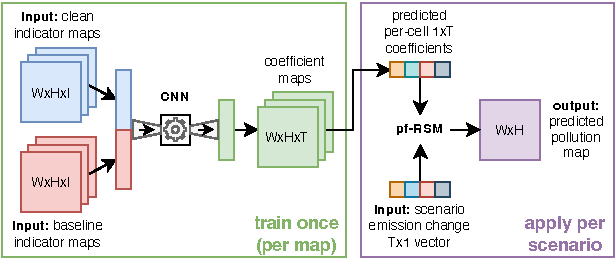
\includegraphics[width=0.9\textwidth]{background/figures/deep-rsm.pdf}
    \caption[Overview of the DeepRSM architecture]{Overview of the DeepRSM architecture. Given the \textbf{W}idth$\times$\textbf{H}eight-sized concentrations maps of \textbf{I} indicators from a baseline and a clean simulation run, the CNN is trained to predict the $1 \times$\textbf{T} per-grid-cell coefficients of the polynomial RSM, pf-RSM. Next, the \textbf{T}$\times 1$-sized emission change vector from an emission control scenario is combined with the coefficients to produce the pollution concentration prediction map output. Please refer to \textcite{deep-rsm-2020} for a detailed description of the layer-by-layer implementation of their CNN.}
    \label{fig:deep-rsm}
\end{figure}

\noindent This concept is borrowed from convolutional neural networks (CNNs), which we briefly describe in this paragraph. CNNs are biologically-inspired shift-invariant networks with a fixed-size footprint that are trained over arbitrary-sized input images by shifting the network over each image \cite{cnn-1990}. The shifting is achieved through convolutional layers, which use convolution instead of matrix multiplication to calculate the layer's outputs \cite{neocognitron-1980}. The convolution layers are interspersed with downsampling layers that progressively increase CNN's receptive field, i.e. the area of inputs that affect each output. Overall, CNNs are characterised by sharing parameters across all shifts, which reduces the number of trainable weights and thus speeds up training and decreases the capacity for overfitting. While CNNs have their origins in 1980 \cite{neocognitron-1980}, they rose in popularity in the 2010s when advances in training neural networks on highly parallel graphics processing units (GPUs) enabled the AlexNet CNN architecture to win the prestigious ImageNet Large Scale Visual Recognition Challenge in 2012 \cite{alexnet-2017}.

\newpar \Cref{fig:deep-rsm} provides a high-level overview of the CNN-based DeepRSM architecture that \citeauthor{deep-rsm-2020} introduce. They build upon the polynomial RSM by \textcite{pf-rsm-2018}, pf-RSM, which is summarised in \Cref{txt:rsm-history}. However, \citeauthor{deep-rsm-2020} strive to fit the polynomial RSM using only the simulation runs for a ``normal'' baseline scenario and a clean air scenario. Note that while this choice drastically reduces the training collection burden, it also reduces the independence of the training data samples, which now only represent the chosen scenarios for a single area. With this reduced dataset, the authors train a deep CCN on the spatial concentrations of 18 indicator species to find the per-cell coefficients $\theta_i$ for the following pf-RSM-inspired polynomial:
\begin{equation*}
    \Delta C = \sum_{i=1}^{N} \theta_i \cdot (E_{\text{NO}_{x}})^{a_i} \cdot (E_{\text{SO}_2})^{b_i} \cdot (E_{\text{NH}_3})^{c_i} \cdot (E_{\text{VOCs}})^{d_i}
\end{equation*}
where $\Delta C$ is the change in concentration for a pollutant, $E_{\text{NO}_{x}}$ is the ratio change in in $\text{NO}_{x}$ emissions, and $a_i$ is a fixed integer power that is determined by the set of polynomial terms used for each pollutant\footnote{For instance, the following $N = 14$ polynomial terms are used to predict $\Delta |\text{O}_3|$: $\text{NO}_{x}$, ${\text{NO}_{x}}^2$, ${\text{NO}_{x}}^3$, ${\text{NO}_{x}}^4$, ${\text{NO}_{x}}^5$, $\text{VOCs}$, $\text{VOCs}^2$, $\text{VOCs}^3$, $\text{NO}_{x} \cdot \text{VOCs}$, $\text{NO}_{x} \cdot \text{VOCs}^3$, ${\text{NO}_{x}}^2 \cdot \text{VOCs}$, ${\text{NO}_{x}}^5 \cdot \text{VOCs}$, $\text{SO}_2$, and $\text{NH}_3$ \cite{deep-rsm-2020}.}. In the final layer of the CNN, the dot product between the learned coefficients $\theta_i$ and the emission change terms is taken to produce the pollutant concentration estimates. During training, the CNN is optimised with the following per-grid-cell loss function \cite{deep-rsm-2020}:
\begin{equation*}
    \mathcal{L}(\hat{y}, y) = \frac{||\hat{y} - y||_1}{y}
\end{equation*}
which penalises high relative concentration errors between the simulated concentration $y$ and the pf-RSM prediction $\hat{y}$. At test time, the concentrations of the indicator species in a baseline and a clean run are passed through the CNN to predict the polynomial coefficients. The effect of a new emission control scenario is then obtained by taking the dot product of the emission change terms and the coefficients. After the CNN has been run on the indicator maps just once, the coefficients for this map can be stored, and any number of new emission control scenarios can be efficiently evaluated by a per-cell dot product. However, a change in the map requires a re-evaluation of the CNN.

\newpar \citeauthor{deep-rsm-2020} make three additional improvements to their deep CNN-based pf-RSM fitting procedure. First, they further increase the amount of training data by randomly cropping the simulation run output maps. Second, the CNN is trained on batches of emission change vectors from different control scenarios. This batching ensures that the deep neural network has to generalise over several diverse scenarios at every gradient backpropagation step. Third, the authors also fit a three-layer fully connected neural network on the emission change vector to produce 50 additional polynomial factors that compensate for effects that the 14-term pf-RSM polynomial cannot capture. This extra `Compensated Polynomial Term' module can thus be seen as a separate error predictor for the pf-RSM module.

The authors demonstrate that their DeepRSM generalises well across different time spans and locations in the same simulation area. They also show that the pre-trained DeepRSM CNN can easily be adjusted for a new application area by retraining it with little new simulation data from the new domain. Thus, DeepRSM can indeed be successfully applied after training on just two simulation runs \cite{deep-rsm-2020}.

\subsection{Integrating Uncertainty with Stochastic RSMs} \label{txt:stochastic-rsm}

How can RSMs integrate the uncertainty of their inputs? \textcite{srsm-phd-1999} further extend RSMs to Stochastic RSMs, SRSMs, which take in random variables as inputs to propagate each input's uncertainty to the output. Similar to pf-RSM, a polynomial is fit to the data, though it is now a combination of random variables instead of observed values. In particular, the authors use a set of independent standard normal random variables $\text{N}(0, 1)$ to represent the uncertainties in all model input variables. Since the output of the SRSM is a polynomial combination of these random variables, the uncertainty in any prediction can be evaluated analytically on the SRSM's polynomial.

\newpar How is an SRSM fit to a model with non-normal-distributed input uncertainties? First, the input distributions are transformed into a set of independent standard normal random variables. For instance, the normal distribution $\text{N}(\mu, \sigma^2)$ and the uniform distribution $\text{U}(0, 1)$ can be obtained from $\text{N}(0, 1)$ as follows \cite{srsm-phd-1999}:
\begin{equation*}
    \text{N}(\mu, \sigma^2) = \sigma \cdot \text{N}(0, 1) + \mu
\end{equation*}
\begin{equation} \label{eq:srsm-uniform}
    \text{U}(a, b) = a + (b-a) \left( \frac{1}{2} + \frac{1}{2} \cdot \text{erf}\left( \frac{\text{N}(0, 1)}{\sqrt{2}} \right) \right)
\end{equation}
\citeauthor{srsm-phd-1999} also provides similar derivations for the lognormal, gamma, exponential, Weibull, and extreme distributions. Continuous distributions with unknown analytical forms can be approximated to a desired accuracy as a weighted sum of several independent normal random variables instead. For empirical distributions where a histogram or its cumulative distribution function $g(x)$ is known, the inverse sampling method can be applied to transform the random variable \cite[p.~28]{rv-generation-1986}:
\begin{equation*}
    x = g^{-1}(u) \quad \text{where} \quad u \sim \text{U}(0, 1) \text{ which is obtained from N}(0, 1){ using \Cref{eq:srsm-uniform}}
\end{equation*}
Since all previously described methods assume independent random variables, the authors also present a transformation for correlated random variables \cite[pp.~42-43]{srsm-phd-1999}, which is not further described here.

\citeauthor{srsm-phd-1999} use polynomial chaos expansion on the selected set $\{\text{N}(0, 1)_i\}_{i=1}^{N}$ of $N$ independent standard normal random variables. Polynomial chaos expansion \cite{polynomial-chaos-1938} refers to the ``series expansion of normal random variables, in terms of Hermite polynomials'' \cite[p.~44]{srsm-phd-1999}, which form ``an orthogonal basis for the space of square-integrable pdfs'' \cite[p.~44]{srsm-phd-1999}:
\begin{equation} \label{eq:polynomial-chaos}
    \begin{split}
        y \approx a_0 &+ \sum_{i_1 = 1}^{N} a_{i_1} \Gamma_1(\xi_1) + \sum_{i_1 = 1}^{N} \sum_{i_2 = 1}^{i_1} a_{i_1,i_2} \Gamma_2(\xi_1, \xi_2) \\ &+ \sum_{i_1 = 1}^{N} \sum_{i_2 = 1}^{i_1} \sum_{i_3 = 1}^{i_2} a_{i_1,i_2,i_3} \Gamma_3(\xi_1, \xi_2, \xi_3) + ...
    \end{split}
\end{equation}
where $y$ is the simulation output that is being approximated, $a_1, a_{1,1}, ...$ are the coefficients whose values are to be determined during fitting, $\{ \xi_1, \xi_2, ..., \xi_N \}$ is the set of $N$ standard normal samples that are obtained from the simulation input $X$ through the aforementioned transformations, and ``$\Gamma_p(\xi_1, ..., \xi_p)$ are multi-dimensional Hermite polynomials of degree $p$'' \cite[p.~45]{srsm-phd-1999}, which are functions of random variables and thus random variables themselves. Please refer to \textcite{polynomial-chaos-1938} and \textcite{polynomial-chaos-1991} for a thorough introduction to polynomial chaos expansion and the Hermite polynomials.

The generated polynomial from \Cref{eq:polynomial-chaos} is fit using collocation, i.e. a system of linear equations is constructed that sets the polynomial equal to the simulation outputs at a set of collocation input points. These systems, which require one simulation result sample per coefficient to fit, can then be solved using any linear solver. For instance, fitting a second-order polynomial chaos expansion requires $N_2 = 1 + 2N + \frac{N(N-1)}{2} = \text{O}(N^2)$ samples, while a third-order expansion already needs $N_3 = 1 + 3N + \frac{3N(N-1)}{2} + \frac{N(N-1)(N-2)}{6} = \text{O}(N^3)$ evaluations to be fit. Since the collocation method finds a polynomial that exactly passes through all collocation points, it is sensitive to the selection of these reference points. The authors present a twofold solution to improve the stability of this process. First, they present a novel `Efficient Collocation Method', which picks collocation points that are closer to the zero-mean of the input standard normal random variables and thus have higher probability. Second, they propose generating twice the number of required samples and then finding the optimal but non-exact polynomial-coefficient solution for the now overdetermined system of linear equations. This fitting process is started with a low-order polynomial chaos expansion and repeated for increasing orders until some user-defined convergence criterion is met. \citeauthor{srsm-phd-1999} note that this general fitting procedure can also be optimised if more insight into the underlying simulation exists. While the process above works on any black box model, known linear transformations of the inputs can be translated analytically, and specific non-linear modules can then be fitted separately.

\newpar \citeauthor{srsm-phd-1999} also explore how the number of samples required to fit the polynomial chaos expansion can be reduced. If auto-differentiation (see \Cref{txt:auto-differentiation}) can be applied to the underlying simulation to automatically calculate the derivative of the simulation output with respect to $M$ simulation input variables, these derivatives can also be plugged into the collocation equations alongside the model outputs:
\begin{equation*}
    \begin{split}
        f(X_i) &= y_i \quad \forall i \in \{0; N\} \\
        \frac{\partial f(X_i)}{x_j} &= d_{i,j} \quad \forall i \in \{0; N\}, j \in \{0; M\}
    \end{split}
\end{equation*}
where $X_i$ is the input for a particular sample, $x_j$ is the $j$th component of the input vector, and $d_{i,j}$ is the partial derivative of the model output with respect to $x_j$ for the input $X_i$ as computed by auto differentiation. Thus, the number of data points per sample increases from $1$ to $1+M$, and the number of samples for the $k$th order polynomial chaos expansion decreases from $2N_k$ to $\frac{2N_k}{M+1}$. 

\textcite{srsm-2004} use the ADIFOR \cite{adifor-1992} auto-differentiation by source-code-transformation tool to fit an SRSM using both model outputs and derivatives. While Stochastic RSMs are built to describe how uncertainty propagates from the inputs to the output, they can also be used to reduce uncertainty. For example, in Bayesian inference, a model's parameter distributions are optimised by maximising the likelihood that this model with these parameters might have produced an observed output. If evaluating the likelihood function is expensive, it can be approximated with an SRSM to speed up inference \cite{srsm-2004}.

\section{Uncertainty Quantification for Model Predictions} \label{txt:uncertainty-quantification}

Machine Learning models are built to approximate often complex and non-linear processes. In most non-toy examples, these models make imperfect predictions. Furthermore, the prediction errors are usually not independently and identically distributed (iid) normal distribution samples from the same error distribution across the entire input domain. Simply trusting the model's point prediction or only reporting some globally-averaged error bounds are insufficient approaches to deal with prediction errors\footnote{If the uncertainty is homoscedastic, i.e. constant across the input space, global error bounds are sufficient. However, uncertainty is often heteroscedastic and varies across the input space.}. Knowing a model's uncertainty is especially relevant in domains where a model's predictions are safety-critical, such as medicine. \textbf{Uncertainty Quantification} is an expanding field in which more than 2,500 papers were published during the last decade \cite{uq-review-2021}. Since this section aims to give only a brief overview of a few methods relevant to this project, please refer to \textcite{uq-review-2021} for a broader review of the field.

\newpar In this section, we denote a model's input as $x$ and the target output it aims to approximate as $y$. Both can be scalar or vectors, but for now, they only represent one input-output sample each. A model with uncertainty quantification outputs two quantities. $\mu(x) \approx y$ is the model's point-approximation for the target output $y$. $\sigma^2(x)$ is the model's uncertainty prediction. If we assume that the model's prediction errors are Gaussian distributed, the model predictions follow the normal distribution $\text{N}(\mu(x), \sigma^2(x))$. However, uncertainty quantification can also be extended to non-normal-distributed errors, e.g. through observing the error distribution across an ensemble (see \Cref{txt:ensembles-decision-tree-random-forest} and \Cref{txt:mc-dropout}). Alternatively, several sub-models can be trained to predict the quantiles of the target function using the pinball loss \cite{regression-quantiles-1978, deep-quantiles-2022}:
\begin{equation*}
    \mathcal{L} = \begin{cases}
        q \cdot \mathcal{L}_{raw} \quad &\text{if } \mathcal{L}_{raw} \geq 0 \\
        (1-q) \cdot \mathcal{L}_{raw} \quad &\text{otherwise}
    \end{cases} \quad \text{where} \quad \mathcal{L}_{raw} = y - \hat{y}_{q}
\end{equation*}

\subsection{Predictive, Aleatoric and Epistemic Uncertainty} \label{txt:aleatoic-epistemic-uncertainty}

The error that a model makes can be quantified as its \textbf{predictive} uncertainty $\sigma^2(x)$. This predictive uncertainty consists of two parts, aleatoric and epistemic uncertainty:

\textbf{Aleatoric} uncertainty originates in the process from which the input data $x$ is sampled. It is thus often described as irreducible. Consider, for instance, modelling a chaotic system such as our weather. Both the measurements, which are taken to predict the weather, and the physical processes that determine it have inherent randomness. Thus, the values of the inputs and the target output carry uncertainty that cannot be reduced and that any model must consider in order to avoid overconfident predictions.

\textbf{Epistemic} uncertainty, on the other hand, comes from the model's lack of knowledge about the process it is modelling. Continuing with the weather example, consider trying to fit a model with few training samples. While low-frequency patterns such as seasonal changes may be learned quickly, the day-to-day or hour-to-hour weather patterns may appear entirely random to the model if it lacks enough data points or variables to learn from. Therefore, several different models can come up with very different predictions, which signifies the ambiguity in how the model should be fit with this limited knowledge. In contrast to the irreducible aleatoric uncertainty, epistemic uncertainty can be reduced by providing a model with more training data, particularly in input regions where the output changes at high frequency.

\newpar How can a model's predictive errors be disentangled into aleatoric and epistemic uncertainty? Splitting the uncertainty is beneficial in several tasks. For instance, in active learning, a model's uncertainty for unseen inputs is used to evaluate for which inputs it would be most beneficial to find the true target outputs to extend the model's training set and improve its performance. However, collecting more training data in regions that are characterised by high aleatoric uncertainty would be of no use since this uncertainty is irreducible. On the other hand, regions of high epistemic uncertainty indicate that the model's predictions may be less trustworthy since it lacks essential knowledge about the processes it attempts to approximate.

\textcite{uncertainty-disentanglement-2022} provide a generalised method to disentangle aleatoric and epistemic uncertainty, which is based on prior work by \textcite{bayesian-deep-uncertainty-2017} for models using Monte Carlo Dropout (see \Cref{txt:mc-dropout}). For their method, the model needs to produce several estimates for its target output and uncertainty predictions. If the model is based on an ensemble (see \Cref{txt:ensembles-decision-tree-random-forest}) of sub-models, their target and uncertainty predictions $\mu_i(x)$ and $\sigma^2_i(x)$ can be taken. If the model is probabilistic, it can be evaluated several times to obtain the iid $\mu_i(x)$ and $\sigma^2_i(x)$ samples. The authors show that the combined predictive uncertainty
\begin{equation*}
    \sigma^2_{\text{predictive}}(x) = \frac{1}{N} \sum_{i=1}^{N} \left( \sigma^2_i(x) + \mu^2_i(x) \right) - \mu^2_{\text{predictive}}(x) \quad \text{where} \quad \mu_{\text{predictive}}(x) = \frac{1}{N} \sum_{i=1}^{N} \mu_i(x)
\end{equation*}
can be rewritten as
\begin{equation} \label{eq:uncertainty-disentanglement}
    \sigma^2_{\text{predictive}}(x) = \text{E}[ \sigma^2_i(x) ] + \text{var}[ \mu_i(x) ] = \sigma^2_{\text{aleatoric}}(x) + \sigma^2_{\text{epistemic}}(x)
\end{equation}

\subsection{Cheap Uncertainty Predictions using Variance Attenuation} \label{txt:variance-attenuation}

How can a model be trained to cheaply output the uncertainty of its target value predictions? \textcite{nll-loss-1994} propose extending a neural network that predicts $\mu(x)$ with a second output for $\sigma^2(x)$. Since the prediction uncertainty is always positive and is never zero in real-world examples, they suggest using the exponential \cite{nll-loss-1994} or softplus \cite{reliable-variance-2019} activation functions, $\exp(x)$ and $\ln(1 + \exp(x))$ respectively, to impose these constraints. If the mean-squared error loss $(\mu(x) - y)^2$ is used to optimise the target value predictions, and a Gaussian prediction error distribution is assumed, the following \textbf{N}egative \textbf{L}og-\textbf{L}ikelihood loss $\mathcal{L}_{NLL}$ optimises the neural network to make the maximum likelihood predictions $y \sim \text{N}(\mu(x), \sigma^2(x))$:
\begin{equation} \label{eq:nll-loss}
    \mathcal{L}_{NLL}(x, y) = \frac{\ln(\sigma^2(x))}{2} + \frac{(\mu(x) - y)^2}{2 \sigma^2(x)}
\end{equation}
This loss function encourages low variance and accurate mean predictions, where possible, by down-weighting the prediction error when high variance is predicted. If the variance predictor captures aleatoric uncertainty well, down-weighting points with high aleatoric can make the network training more robust to outliers \cite{bayesian-deep-uncertainty-2017}.

\newpar However, the variance attenuation loss $\mathcal{L}_{NLL}$ also has two problems. First, it is prone to overconfidence, i.e. predicting too-low variance \cite{reliable-variance-2019}. If the mean and variance predictor are trained together, the predicted variance is encouraged to approach zero since the target value predictions on the training data set keep improving \cite{variational-variance-2020}. However, since $\mathcal{L}_{NLL}$ in \Cref{eq:nll-loss} divides the prediction error $(\mu(x) - y)^2$ by $2 \sigma^2(x)$, minor prediction errors lead to large loss gradients when the predicted variance approaches zero, which makes the training process unstable. \textcite{reliable-variance-2019} propose, amongst others, two simple solutions to alleviate the overconfidence problem. Suppose the input dimensionality is low enough that nearest-neighbour distances are meaningful. In that case, the authors suggest extending each training batch of $(x_i, y_i)$ pairs to also include the nearest neighbours of each $x_i$ to ensure that each batch contains information about both the target value mean and variance. Alternatively, training the mean and variance should be separated. After the network has been trained to predict $\mu(x)$ assuming constant predictive variance, the variance prediction is trained using the no-longer-updated mean predictions. This design also invites separating $\mu(x)$ and $\sigma^2(x)$ into two separate neural networks. Note that there are also more radical approaches to alleviate the variance overconfidence problem, including assuming Student's $t$ distributed errors \cite{reliable-variance-2019} or modelling variance variationally \cite{variational-variance-2020}, which are omitted here for brevity.

\newpar The second problem of the variance attenuation loss comes from its down-weighting of training samples with high predicted variance. While it is expected that the network may just predict the global mean value with high uncertainty during early training, there is the danger of the model getting stuck in such suboptimal predictions. In particular, if slightly more difficult points are always down-weighted, the model may never attempt to learn to predict them and thus perform much worse than a model trained only to output the target values but not the predictive variance. \textcite{beta-nll-2022} propose the following $\beta$-NLL loss to overcome this issue:
\begin{equation}
    \mathcal{L}_{\beta-NLL}(x, y) = \text{stop}(\sigma^{2 \beta}(x)) \cdot \mathcal{L}_{NLL}(x, y) \label{eq:beta-nll-loss}
\end{equation}
where $\beta \in [0; 1]$ is a newly introduced hyperparameter and the $\text{stop}(expression)$ function stops the gradient coming from the contained $expression$ from participating in the gradient backpropagation of the neural network (see \Cref{txt:neural-network}). As $\beta$ approaches zero, the $\beta$-NLL loss reduces to the original NLL loss. As $\beta$ approaches one, the gradient of the $\beta$-NLL loss with respect to the target value prediction $\mu(x)$ becomes equivalent to the gradient in the mean-squared error loss, where every training sample is given equivalent weight. The authors recommend $\beta = 0.5$ since it weights the samples with the ``inverse standard deviation instead of [the] inverse variance'' \cite{beta-nll-2022} and ``achieves the best trade-off between accuracy and log-likelihood'' \cite{beta-nll-2022}.

\subsection{Built-in Uncertainty with Gaussian Process Models} \label{txt:gaussian-process}

Gaussian Processes (GPs) are stochastic processes that fit a multivariate normal distribution to a training dataset. Specifically, GPs consist of a collection of random variables (RVs), where any linear combination of the RVs follows some multivariate normal distribution $\mathcal{N}(\mu, \Sigma)$ \cite{gp-ml-2005}. A GP that represents a process $f(x)$ is denoted as \cite{gp-ml-2005}:
\begin{equation*}
    f(x) \sim \mathcal{GP}(m(x), k(x, x')) \sim \mathcal{N}(\mu, \Sigma)
\end{equation*}
where $m(x)$ is the GP's mean function, $k(x, x')$ represents the GP's covariance, $x'$ is any input from the training data $X_{train}$, and $x$ is any input from the input domain. It is often assumed that the Gaussian Process has zero mean and is thus only defined by its covariance. The covariance can be split into a covariance kernel $K(X, X)$ and observation noise $\sigma^2 I$. The kernel notation $K(X, X)$ is a shorthand for the matrix of pairwise covariances, where each entry $k_{i,j}$ is calculated using the kernel function $k(x_i, x_j)$ \cite{rio-2019}. Commonly used kernel functions that we refer to in this thesis include:
\begin{enumerate}
    \item \textbf{Constant:} $k(x_i, x_j) = \sigma^2$
    \item \textbf{White Gaussian Noise:} $k(x_i, x_j) = \begin{cases}
        \sigma^2 &\quad \text{if } i = j \\
        0 &\quad \text{otherwise}
    \end{cases}$
    \item \textbf{Radial Basis Function (RBF):} $k(x_i, x_j) = \exp{\left( -\frac{||x_i - x_j||_2}{2 \sigma^2} \right)}$
    \item \textbf{Sum Kernel:} $k(x_i, x_j) = k_1(x_i, x_j) + k_2(x_i, x_j)$ where $k_1(x_i, x_j)$ and $k_2(x_i, x_j)$ are kernel functions
\end{enumerate}
\noindent When selecting the Gaussian Process kernel, knowledge about the problem domain can be used to compose a kernel that reflects the expected components of the real-world process. Next, the zero-mean GP is fit by optimising the log marginal likelihood of the covariance kernel. Finally, the fitted GP can be used to predict multivariate normal distributions for unseen inputs \cite{gp-ml-2005}:
\begin{equation*}
    \begin{split}
        Y_{test} \given X_{train}, Y_{train}, X_{test} &= \mathcal{N}(\mu(X_{test}), \Sigma(X_{test})) \quad \text{where} \\
        \mu(X_{test}) &= K(X_{test}, X_{train}) \times [K(X_{test}, X_{test}) + \sigma^2 I]^{-1} \times Y_{test} \\
        \Sigma(X_{test}) &= K(X_{test}, X_{test}) - K(X_{test}, X_{train}) \times [K(X, X) + \sigma^2 I]^{-1} \times K(X_{train}, X_{test})
    \end{split}
\end{equation*}
\noindent By sampling from these predicted multivariate normal distributions $M$ times for a range of input points $x$, the evaluations of $M$ plausible \textit{functions} that explain the training data can be sampled \cite{gp-ml-2005}:
\begin{equation*}
    f_i(x) \sim \mathcal{N}(\mu(x), \Sigma(x)) \quad \text{where} \quad x \in X \text{ and } i \in \{1, ..., M\}
\end{equation*}
\noindent It is worth noting that prediction requires calculating the inverse of the covariance matrix, which has cubic complexity and is thus infeasible for large training datasets. Therefore, approximation methods are often used in practice. For instance, the training data set can be randomly or greedily \cite{gp-ml-2005} subsampled. More complex methods include Stochastic Variational GPs \cite{svgp-2013}, which use a reduced set of trainable inducing variables, and Actually Sparse Variational GPs \cite{asvgp-2023}, which project the GP onto a set of B-spline basis functions. Please refer to \textcite{big-data-gp-2022} for their classification and evaluation of GP approximation methods.

\subsection{Ensemble Uncertainty and Monte-Carlo Dropout} \label{txt:mc-dropout}

Predictive uncertainty can be decomposed into irreducible aleatoric uncertainty and model-based epistemic uncertainty (see \Cref{txt:aleatoic-epistemic-uncertainty}). Since aleatoric uncertainty is irreducible, several independent models should be able to measure it equivalently. In contrast, epistemic uncertainty describes the variation across different models that can explain the same observations with different theories but with equivalent accuracy. Put simply, epistemic uncertainty should be high if vastly different models can explain the data, and low if the models are forced to converge on a single hypothesis. Thus, it is intuitive to measure epistemic uncertainty as the spread of predictions across the models of an ensemble (see \Cref{eq:uncertainty-disentanglement}).

\newpar \Cref{txt:ensembles-decision-tree-random-forest} has already summarised why ensembles can make better predictions than the models they consist of \cite{ml-ensembles-2000}. Since ensembles thus provide benefits for both prediction and uncertainty quantification, ensembles have been extensively applied in recent years, e.g. \cite{mc-dropout-2016, deep-ensembles-2017, ensemble-uncertainty-2021, ensemble-diversity-2015, ensemble-uncertainty-ood-2021}. While this subsection provides a very brief overview of ensemble-based uncertainty quantification, please refer to \textcite{ensemble-uncertainty-2021} for a more extensive investigation of the topic.

\textcite{deep-ensembles-2017} introduce deep ensembles, which train an ensemble of neural networks (see \Cref{txt:neural-network}) with randomised initial parameter values and shuffled training data points. \textcite{ensemble-diversity-2015} have specifically highlighted the importance of diversity when training ensembles. They show that training over different random initialisations can be more potent than simply resampling the training dataset for each ensemble member. The authors also found that diversity is particularly advantageous in higher-level layers closer to the output. Thus, \citeauthor{ensemble-diversity-2015} introduced TreeNets as a compromise solution between fully independent and fully parameter-sharing ensemble members. TreeNets only share the first few neural network layers, followed by multiple distinct branches that make independent predictions.

Another approach, Monte Carlo Dropout by \textcite{mc-dropout-2016}, is based on dropout. Dropout was initially introduced by \textcite{dropout-2014} as a technique to reduce overfitting in neural networks. In particular, layers that use dropout randomly drop some of their outputs during training with probability $p$. Therefore, in every forward propagation through the network, only a fraction of the neurons are active, which leads to faster computation times for large networks. Furthermore, it forces the network to be robust to the failure of individual neurons, making it less likely to overfit. At evaluation time, no neurons are dropped, but all weights are multiplied by the factor $p$. Monte Carlo Dropout builds on this idea but also applies random dropout at prediction time. Since predictions are now random, the network can be sampled several times to obtain an ensemble of predictions and evaluate its uncertainty. \citeauthor{mc-dropout-2016} have shown that using Monte Carlo sampling on a network with dropout ``approximate[s] Bayesian inference in deep Gaussian processes'' \cite{mc-dropout-2016}.

% Andreas: Words with mathematical meaning should be defined on the first usage. Inconcise notation cannot be mixed with the use of mathematical properties lacking a concise definition. In addition, the mathematical citation style puts less emphasis on the author names.
\section{Avoiding Overconfidence using Novelty Detection} \label{txt:novelty-detection}

In machine learning, the closed-world assumption is generally assumed to hold. That is, a model's training data is assumed to be drawn independently and identically distributed (iid) from the same distribution as the test data and the data on which the model is later applied \cite{ood-boundary-2021}. Put simply, if we want a machine learning model to approximate some target function, the training data must cover \textbf{all} aspects of the possible input data sufficiently well. However, this assumption may not always hold.

\newpar For an easy and illustrative example, consider a model that is trained to distinguish between pictures of apples and bananas. However, during training, it is only shown pictures of green apples and pictures of yellow bananas. With such a limited training data set, the model might learn to associate apples only with the colour green, and bananas only with the colour yellow. What happens if the model is shown a red apple at test time? The closed-world assumption is clearly violated here since the model was never trained on red apples. Thus, the model might fail on this input in an unpredictable way and without any indication. This example is easy to catch: Since the model was never trained on any red fruit at all, it could refuse to make a prediction.

So what should the model do if it is shown a yellow apple and a green banana? Given its limited training, the model might mistake the apple for a banana and vice versa. Since the model has been trained on both apples and bananas and both the colours yellow and green, how could it have detected that it should not have made a prediction in this case either? During its training on the images of green apples and yellow bananas, the model likely observed both the colour and rough shape of each fruit but decided -- for simplicity -- to assume that all green fruit are around are apples and that all yellow fruit are crescent-shaped are bananas. When the model is then presented with a yellow but round fruit, the model's learned assumption that all yellow fruits are crescent-shaped is violated. If it can detect this assumption violation, the model can correctly determine that it should not make a prediction for yellow apples and green bananas.

\newpar To decide whether a model can make a prediction, one has to check whether a new input is similar to the inputs that the model was trained on. Inputs that the model was trained on are called \textbf{ID}, short for \textbf{in-distribution}, while inputs that come from a different distribution are called \textbf{OOD}, short for \textbf{out-of-distribution}. Deciding if an input is ID or OOD is an application of \textbf{novelty detection}. This machine learning task aims to identify novel inputs, anomalies, outliers, or exceptional data points amongst a set of ``normal'' data. As an unsupervised task, it is only presented with such ``normal'' ID data but no OOD examples during training \cite{novelty-detection-2010}. Thus, novelty detection can be phrased as a one-class classification problem \cite[e.g.][]{ood-svm-1999}.

Novelty can occur at different scales \cite{novelty-detection-2010}. For example, a subset of data can be novel on a population scale if it follows a different distribution. Likewise, in a time series or a geographical map, individual data points can be novel in the context of their surrounding points. Such coarser-scale shifts in the data distribution can be identified using \textbf{concept drift} detection methods, which are discussed in further detail in \Cref{txt:concept-drift}. For individual points without context, however, an independent decision must be made for every single data point without being able to compare them to nearby points or population statistics. Building on the broad overview provided by \textcite{novelty-detection-2010}, the following subsections describe a variety of novelty detection methods in detail.

\subsection{A brief Overview of Concept Drift} \label{txt:concept-drift}

Before we dive into novelty detection methods for individual outlier points, we briefly summarise concept drift. Concept drift describes an unforeseen change \cite{concept-drift-definition-2019} in the distribution of input-output samples $(X, Y)$ across a contextual subsample, e.g. a period in time. Hence, concept drift deals with population-level changes in a distribution and does not consider individual outliers. Whereas individual-based methods can be applied to contextless individuals and data points from a population sample, concept drift methods only work on population samples. Thus, they can incorporate more information. For instance, a concept drift detector may not detect a single red apple amongst many green ones. However, it could detect if an apple's colour slowly changes from green to yellow over several images.

\newpar \textcite{concept-drift-definition-2019} formally define the existence of concept drift, which starts at a time point $t$ and spans a time window $w$, as
\begin{equation*}
    \exists t \st P_t(X, Y) \neq P_{t+w}(X, Y) \quad \text{where} \quad P_t(X, Y) = P_t(X) \cdot P_t(Y \given X)
\end{equation*}
where $P_t(X, Y)$ is the observed input-output distribution at time $t$, $P_t(X)$ is the input distribution at time $t$, and $P_t(Y \given X)$ is the output label posterior distribution given input $X$ at time $t$. This definition neatly distinguishes the three kinds of concept drift. \textbf{Virtual or feature drift} occurs when the input distribution $P_t(X)$ changes but the relationship to the output remains the same, e.g. when for a linear model $f(x) = 2x + 8$ the data samples shift from $\{ (1, 10), (2, 12), (3, 14) \}$ to $\{ (2, 12), (4, 16), (6, 20) \}$. \textbf{Real concept drift} occurs when the posterior $P_t(Y \given X)$ shifts but the input distribution remains the same, e.g. when $f_t(x) = 2x + 8$ changes to $f_{t+w}(x) = 3x + 8$ for the input distribution samples $\{ 1, 2, 3 \}$. Finally, both input and posterior distribution can also shift simultaneously. \textcite{concept-drift-rates-2014} further differentiate various concept drift types by the rate at which they occur. For instance, the drift can be abrupt, occur in incremental steps with intermediate concepts, gradually interpolate between the old and the new concept, or be recurring.

\newpar \textcite{concept-drift-detectors-2022} provide a comprehensive overview of the many proposed concept drift detection algorithms, which the authors classify into several categories. \textbf{Data-distribution-based} methods only observe the distribution of the input-output samples $\{(X_1, Y_1), (X_2, Y_2), ...\}$. These methods can further be restricted to only having access to the distribution of input samples $\{X_1, X_2, ...\}$. In that case, data-distribution-based methods can identify concept drift without needing access to the true output labels $\{Y_1, Y_2, ...\}$ or a machine learning model's predictions for the labels. \textbf{Performance- or error-based} methods instead monitor the prediction error of a model to determine when its performance no longer matches its training accuracy. While these methods, which can be based on model ensembles, comparison windows across time, or statistical significance tests \cite{concept-drift-detectors-2022}, only sound the alarm when a model actually starts to make consistent mispredictions, they \textbf{always} require access to the true output labels $\{Y_1, Y_2, ...\}$, which may not be available (yet). Finally, several detectors can also be combined in \textbf{hybrid} ensemble methods (see \Cref{txt:ensembles-decision-tree-random-forest}).

\subsection{A Baseline for OOD Detection in Classification} \label{txt:softmax-confidence}

Next, we discuss how the performance of an OOD input detector can be evaluated. \textcite{ood-baseline-2016} introduce a baseline method, which other OOD detection methods for classification can be compared against, and discuss which metrics should be used to measure their performance.

\newpar In classification tasks, the final layer of a neural network is usually a softmax activation function that scales the classification scores for each class into pseudo-probability scores that are non-negative and add up to one. For a specific class $c_i$ amongst all $N$ classes, the softmax activation $S_i(X)$ is defined for the input $X$ and the class scoring functions $f_i(X)$ as follows:
\begin{equation} \label{eq:softmax}
    S_{i}(X) = \frac{e^{f_i(X)}}{\sum_{j=1}^{N}e^{f_j(X)}}
\end{equation}
However, directly interpreting such softmax scores as classification probabilities often leads to highly overconfident predictions on out-of-distribution inputs, e.g. having $91\%$ confidence that Gaussian noise is an image of a particular handwritten digit \cite{ood-baseline-2016}. We further define the maximum softmax score as
\begin{equation} \label{eq:max-softmax}
    S_{c}(X) = \text{max}_{i} \{ S_{i}(X) \}
\end{equation}
i.e. the highest softmax score, or phrased differently, the score for the predicted class $c$. \citeauthor{ood-baseline-2016} show that this maximum softmax score $S_{c}(X)$ is more informative than an arbitrary $S_{i}(X)$, as the maximum score is usually lower for OOD inputs than for ID inputs. Put simply, classification models tend to assign ID inputs to one clear class but are more ambiguous for OOD inputs. The authors show that using a threshold to distinguish between ID and OOD inputs based on $S_{c}(X)$ thus performs well. They also present an auto-associative network-based abnormality detector as a first improvement to their method. Auto-associative networks are discussed in further detail in \Cref{txt:auto-associative}.

\newpar Like many other methods, the above baseline OOD detector relies on a threshold to distinguish between ID and OOD samples. \citeauthor{ood-baseline-2016} suggest using the threshold-selection-independent AUC-ROC and AUC-PR metrics to evaluate the performance of a detector method across all possible thresholds. Before introducing these metrics, the following commonly known terms need to be defined, here in the context of OOD detection:
\begin{enumerate}
    \item An OOD detector $d(X)$ classifies an input $X$ as either ID or OOD. For now, we designate OOD as a positive prediction and ID as a negative one, though the reverse is also possible.
    \item The \textbf{true positive rate} or \textbf{recall} $TPR = RC = \frac{|d(X_{\text{OOD}}) = \texttt{OOD}|}{|X_{\text{OOD}}|}$ is the percentage of actual OOD inputs that are correctly identified as OOD.
    \item The \textbf{true negative rate} $TNR = \frac{|d(X_{\text{ID}}) = \texttt{ID}|}{|X_{\text{ID}}|}$ is the percentage of actual ID inputs that are correctly identified as ID.
    \item The \textbf{false positive rate} $FPR = \frac{|d(X_{\text{ID}}) = \texttt{OOD}|}{|X_{\text{ID}}|}$ is the percentage of ID inputs that are mistakenly identified as OOD.
    \item The \textbf{false negative rate} $FNR = \frac{|d(X_{\text{OOD}}) = \texttt{ID}|}{|X_{\text{OOD}}|}$ is the percentage of OOD inputs that are mistakenly identified as ID.
    \item The \textbf{precision} $PR = \frac{|d(X_{\text{OOD}}) = \texttt{OOD}|}{|d(X_{\text{ID}} \cup X_{\text{OOD}}) = \texttt{OOD}|}$ is the percentage of OOD classifications that are correct amongst all ID and OOD inputs that are classified as OOD.
\end{enumerate}
Both the AUC-ROC and AUC-PR metrics calculate the \textbf{A}rea \textbf{U}nder the \textbf{C}urve of two metrics that the threshold has to find a trade-off for. For AUC-ROC, these are the true positive rate and the false positive rate. For AUC-PR, the precision and recall metrics are used instead, which \textcite{aucpr-informative-1999} deem to be more informative, e.g. when ID and OOD inputs are unbalanced. While AUC-ROC scores are independent of whether ID, or as above, OOD inputs are designated as positive, the AUC-PR scores are not and must be reported for both cases \cite{ood-baseline-2016}. \Cref{fig:auc-roc-pr} shows the AUC-ROC and AUC-PR curves for different classifiers. While a random detector obtains an AUC-ROC score of $0.5$, a perfect detector would get AUC-ROC and AUC-PR scores of $1.0$. The AUC-PR score of a random detector depends on the positive-negative class imbalance.

\begin{figure}[ht]
    \centering
    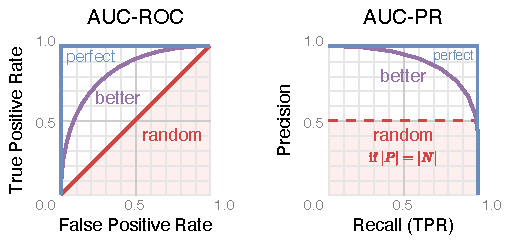
\includegraphics[width=0.9\textwidth]{background/figures/auc-roc-pr.pdf}
    \caption[Examplary AUC-ROC and AUC-PR score curves.]{Examples of AUC-ROC and AUC-PR score curves. While the AUC-ROC score of a random classifier is always $0.5$, the AUC-PR score depends on the rate of positive and negative examples.}
    \label{fig:auc-roc-pr}
\end{figure}

\noindent \textcite{odin-detector-2017} build on \citeauthor{ood-baseline-2016}'s baseline with their \textbf{O}ut-of-\textbf{DI}stribution detector for \textbf{N}eural networks, ODIN. They improve the softmax score with temperature scaling and anti-adversarially perturbed inputs to further push the softmax scores of ID and OOD inputs apart. In contrast to the softmax function as defined in \Cref{eq:softmax}, ODIN scales the scoring function outputs $f_i(X)$ by the inverse of a temperature parameter $T$: 
\begin{equation*}
    S_i(X; T) = \frac{e^{\frac{f_i(X)}{T}}}{\sum_{j=1}^{N}e^{\frac{f_j(X)}{T}}}
\end{equation*}
The $T$-dependent maximum softmax score is defined as $S_{c}(X;T) = \text{max}_{i} \{ S_{i}(X;T) \}$, following \Cref{eq:max-softmax}. The authors show that higher temperatures push ID and OOD scores further apart but that $T > 100$ brings no further benefits. To further increase the separation, \citeauthor{odin-detector-2017} suggest using the fast gradient sign method \cite{fast-gradient-2014} to perturb the inputs before feeding them through the classification network. Counterintuitively, they apply the FGSM to push an input \textbf{towards} its predicted class to increase the confidence in this prediction. Crucially, the authors observe that the increase in confidence is larger for ID than for OOD inputs. Both the temperature scaling and input perturbation are configured such that thresholding on the ODIN softmax scores achieves a true positive rate of $95\%$ on a held-out validation set that was not used during training.

\subsection{Distance-based Methods for Novelty Detection} \label{txt:ood-distance}

Intuitively, a machine learning model should perform well on inputs that are close to the inputs it was trained on. Several methods are built on this intuition to separate ID from OOD inputs. Many methods are based on the simple idea of constructing a bounding volume that includes most of the ID training data points. New inputs that lie on the inside of this volume are ID, while those on the outside are OOD. For instance, the Mahalanobis distance can be used to define a hyper-ellipsoid bounding volume by assuming that the ID data comes from a multivariate normal distribution \cite{mahalanobis-distance-1936, mahalanobis-outlier-2000}:
\begin{equation} \label{eq:mahalanobis-distance}
    d_{M}(x) = \sqrt{(x - \mu_{\text{ID}})^{\intercal} S^{-1}_{\text{ID}} (x - \mu_{\text{ID}})}
\end{equation}
where $d_{M}(x)$ is the distance between an input feature vector $x$ and the ID distribution, and $\mu_{\text{ID}}$ and $S_{\text{ID}}$ are the mean and covariance of the ID training data, respectively. Since the feature distances on the raw high-dimensional inputs are vulnerable to noise and difficult to interpret, the distances are often instead computed on higher-level and lower-dimensional embeddings, e.g. created by the upstream levels of a neural network.

\newpar \textcite{ood-adversarial-detection-2018} fit Gaussian mixture models (GMMs), i.e. weighted sums of multivariate normal distributions \cite{gmm-encyclopedia-2009}, to the training data embedding created by each layer. To classify an unseen input, they then select the class that the input is closest to based on their Mahalanobis distance. After perturbing the input's embedding in this layer adversarially away from the chosen class using the fast gradient sign method \cite{fast-gradient-2014}, the Mahalanobis distance is measured again and translated into a per-layer confidence score ${c}_{i}(x)$ that captures how well the input $x$ lies within the Gaussian fit of the class distribution in this layer. Finally, the parameters $\{ \beta_0, \beta_1, ... \}$ of a logistic regression model are fit on validation data to distinguish between ID and OOD inputs:
\begin{equation*}
    d(x) = \begin{cases}
        \texttt{ID} \quad & \text{if } s(x) < threshold \\
        \texttt{OOD} \quad & \text{otherwise}
    \end{cases} \quad \text{where} \quad s(x) = \frac{1}{1 + e^{-(\beta_0 + \sum_{i}\beta_i \cdot {c}_{i}(x))}}
\end{equation*}
\textcite{ood-class-2022} follow up on this work and suggest integrating OOD detection directly into the classification network by having a separate OOD class. However, they only fit a GMM on the penultimate layer of the neural network since earlier layers may not be normal-distributed. The final classification into either one of the original classes or the new OOD class is then based on the Mahalanobis distance on the penultimate layer. Note that both of these methods require training on OOD inputs, which can come from OOD datasets or be generated synthetically, which \Cref{txt:ood-input-generation} explores in further detail. \citeauthor{ood-class-2022} observe that training their OOD-class detection method generalises well to unseen OOD data even if only a small OOD dataset or just noise as synthetic OOD data is used during training.

\newpar The \textbf{DI}stance to \textbf{M}odelled \textbf{E}mbedding (DIME) is an alternative method by \textcite{dime-detector-2021}. As in the above methods \cite{ood-adversarial-detection-2018, ood-class-2022}, the authors use an upstream layer to investigate the distances in a learned higher-level embedding. First, they fit a linear hyperplane using truncated singular value decomposition such that the ID training data can be reconstructed from its projection onto the hyperplane at minimal loss. The degree of truncation is selected based on how much of the variation in the ID data should be retained. Next, a held-out validation set of ID data points is used to record the distribution of the reconstruction errors. To classify an unseen point $X_i$, the distance $\text{DIME}(X_i)$ between $X_i$'s embedding in the layer and the reconstruction of this embedding from the hyperplane projection is compared to the validation set's reconstruction error distribution -- OOD inputs likely have larger reconstruction errors than ID inputs. The authors propose the following layer-specific score to calculate the probability that a new input $X_i$ comes from the ID input distribution $\mathbb{P}_{\text{ID}}$:
\begin{equation} \label{eq:dime-id-percentile}
    P(X_i \in \mathbb{P}_{\text{ID}}) = 1 - \text{Percentile}_{valid}(\text{DIME}(X_i))
\end{equation}
\citeauthor{dime-detector-2021} also note that DIME can be combined with the Mahalanobis distance, e.g. to measure the distance between the projections of two embedded data points onto the hyperplane, which then also takes the correlations within the training data and distance to the ID distribution on the hyperplane into account. Thus, this extension addresses the method's weakness that a point on the infinite hyperplane is classified as ID, even if it is far away from the projections of all training points. However, it is worth noting that DIME and its extension using the Mahalanobis distance are still limited by only looking at the distances within an upstream embedding layer, where a neural network might already rely on some of its closed-world assumptions. In the previous fruit classification example, DIME would likely recognise a red apple as an OOD input since its hyperplane was not fit to preserve any colours other than green or yellow. However, if, as assumed in the example, the network has already reduced each fruit to just its colour in this layer, DIME would not be able to detect yellow apples or green bananas as OOD inputs since their embeddings would both lie on the ID hyperplane.

\newpar The k-Nearest Neighbour (kNN) algorithm is a method that is used to find the $k$ training inputs that are closest to an unseen input, where $k$ is a hyperparameter\footnote{While the parameters of a model are variables that are optimised during training, hyperparameters configure the training process or model architecture itself. Thus, multiple training runs are required to find the optimal hyperparameter values.}. While kNN is most commonly used for clustering, it can also be applied for novelty detection. For instance, if the mean distance to the $k$ nearest neighbours, or some different property of the graph connecting them \cite{knn-outlier-2004}, exceeds a threshold, the input is considered OOD \cite{novelty-detection-2010}. Similarly, the local outlier factor \cite{lof-outlier-2000}, which estimates the local training data density, can be used to differentiate between areas of high density, i.e. with many ID inputs, and areas with low density where a point is likely OOD. Suppose the input data points can be naturally assigned to clusters. In that case, another approach is to train a clustering algorithm on the ID data and to later assign each new unseen input a membership score for each cluster. Inputs that clearly belong to one cluster are assumed to be in-distribution. In contrast, inputs whose membership approaches the uniform distribution are determined to be out-of-distribution \cite{cluster-novelty-2008}, similar to \citeauthor{ood-baseline-2016}'s baseline detector. It is worth noting that these methods need to keep around \textbf{all} training data samples so that the nearest neighbours can be determined.

\newpar \textcite{distance-confidence-2017} present a distance-based confidence score that can be appended to an existing classification neural network. Instead of measuring the distance between the inputs, the authors look at changes in the embedding created by an upstream layer, i.e. one that is close to the output layer and encodes high-level features. In particular, they compute the embedding distances to the $k$ nearest neighbours among the training points and compare the distances for points with the same class as the predicted one against all neighbour distances. If no nearby points are of the same class or these are all far away, the score approaches zero confidence, while a confidence of $100\%$ is achieved if all $k$ nearest neighbours in the embedding space are of the same class. During training, the model's loss function is augmented such that points of the same class are pulled together in the embedding space, whilst points of different classes are pushed apart. This class separation in embedding space is further encouraged by using the fast gradient sign method \cite{fast-gradient-2014} to generate adversarial inputs that are close to the ID inputs but are of different classes.

\newpar Many of the methods mentioned above are applied to upstream neural network layers since the distances between higher-level features often hold more meaning than the distances between the raw high-dimensional inputs. Alternatively, problem-domain-specific feature space transformations or distance functions can be used. Despite this flexibility, distance-based methods still share the limitation that they assume that distance alone can decide if an input comes from the ID distribution. This assumption may make sense if a machine learning model is only trusted to interpolate between several nearby training data points. However, suppose a model is trained to learn more broadly applicable concepts, e.g. to replicate some laws of physics. In that case, extrapolation within the structure of the ID inputs is desirable.

\subsection{Detecting broken Assumptions using Auto-Associative Networks} \label{txt:auto-associative}

Auto-associative networks are neural networks that learn a mapping $f(X) = X$, i.e. to map the input $X$ to itself \cite{auto-associative-2001}. \Cref{fig:auto-associative-overview} provides an overview of their architecture. Auto-associative networks first reduce the dimensionality of the input $X$ to a compressed bottleneck representation $x$ before increasing the dimensionality again to reconstruct the input $X$ from the bottleneck $x$. Thus, they are encoder-decoder networks trained to find a compressed representation of $X$, $x$, that can be decompressed with minimal error. Suppose the encoding and decoding layers of an auto-associative network use non-linear activation functions with a range of $[0; 1]$, such as the sigmoid function $s(x) = \frac{1}{1 + e^{-x}}$. In that case, they can fit any non-linear function ``with support in the unit hypercube'' \cite{non-linear-pca-1989}. Thus, auto-associative networks can be seen as an implementation of truncated non-linear principal component analysis (PCA)\footnote{Note that if the encoding and decoding layers are removed or use linear activation functions, the auto-associative network instead learns to produce the truncated linear PCA encoding \cite{auto-associative-2001}.} \cite{auto-associative-2001}. When trained on ID data only, they learn the structure of the ID data and find a compression and decompression scheme that removes any redundancy within.

\begin{figure}[ht]
    \centering
    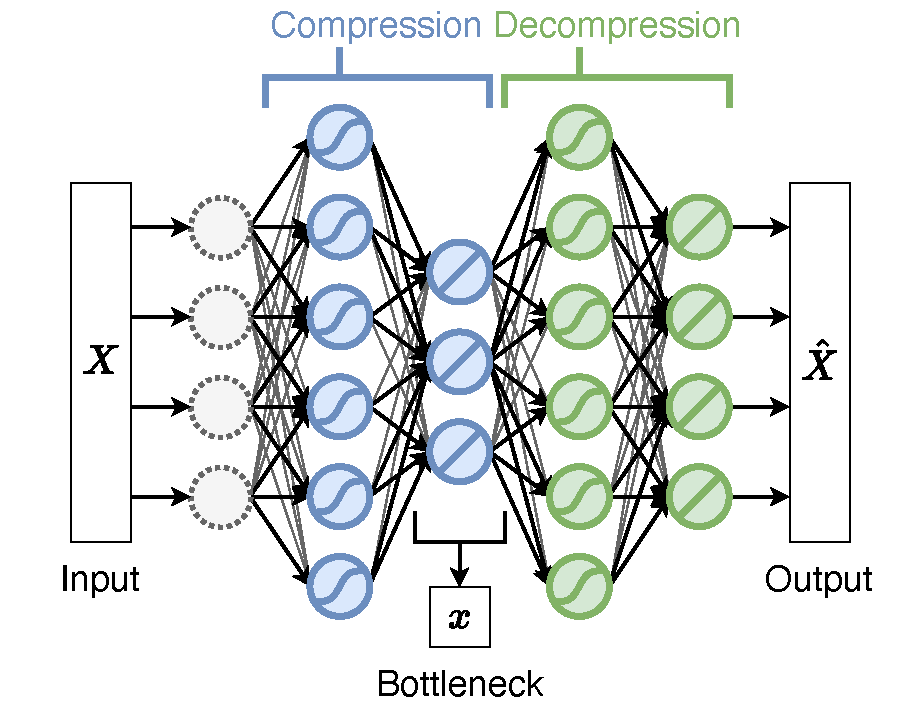
\includegraphics[width=0.84\textwidth]{background/figures/auto-associative.pdf}
    \caption[Overview of an Auto-Associative Network]{Overview of a non-linear Auto-Associative Network. For compression, which is coloured in blue, the input $X$ is first fed through a sigmoid-activated encoding layer and is then compressed to a lower-dimensional bottleneck representation $x$ using a linear activation. For decompression, which is coloured in green, the bottleneck representation $x$ is fed through a sigmoid-activated decoding layer and is then decompressed using a linear activation into $\hat{X}$, approximating $X$. The activation function used by each neuron is indicated symbolically. This schematic is inspired by Figure 1 in \textcite{auto-associative-2001}.}
    \label{fig:auto-associative-overview}
\end{figure}

\noindent In the fruit classification examples, an auto-associative network might learn that round fruit are green whilst crescent-shaped fruit are yellow, and thus encode each fruit only by its colour. During the decoding step, it would then use this learned assumption to reconstruct green fruit as round and yellow fruit as crescent-shaped. Given the limited training data in this example, such a simple auto-associative network would perform very well on ID data of green apples and yellow bananas. However, how would it deal with pictures of yellow apples and green bananas? The encoding step would function as usual and extract only the fruit's colour. However, during decoding, the network would reconstruct erroneously and translate the \textit{yellow} apple into a \textit{yellow} banana and the \textit{green} banana into a \textit{green} apple. The magnitude of such an auto-associative network's reconstruction error, which can be measured as the squared residuals between the input $X$ and the output prediction $\hat{X}$, can thus be used to differentiate between ID and OOD inputs.

\newpar How does one decide on the dimensionality of the bottleneck and the encoding and decoding layers? Setting either too small may cause the network to be unable to replicate the structural complexity within the data and thus force it to make a high-bias underfit. In contrast, making the hidden layers of the auto-associative network too big may allow the network to overfit by memorising some of the natural (random) variance in the data. Instead, \textcite{auto-associative-2001} suggest finetuning the dimensionality hyperparameters by minimising complexity-relative error metrics such as Akaike's Final Prediction Error FPE \cite{akaike-fpe-1969, akaike-fpe-1970, akaike-fpe-1971}, or Akaike's Information Criterion AIC \cite{akaike-aic-1974}, which \citeauthor{auto-associative-2001} specialise for auto-associative networks as:
\begin{equation*}
    FPE = \frac{E}{2N} \cdot \frac{1 + \frac{W}{N}}{1 - \frac{W}{N}}
\end{equation*}
\begin{equation*}
    AIC = \ln{\left(\frac{E}{2N}\right)} + 2 \cdot \frac{W}{N}
\end{equation*}
where $E$ is the auto-associative network's squared prediction error, $W$ is its number of trainable weights, and $N$ is the number of input values \cite{auto-associative-2001}.

\newpar As the auto-associative network learns to compress the input data into a lower-dimensional form, it transforms highly correlated features into a smaller set of independent features. Training a machine learning model on this compressed feature vector $x$ instead of the higher-dimensional input $X$ has two clear advantages. First, it reduces the computational burden of training and evaluating the prediction model. Second, it helps models, like linear regression, that struggle with collinear features \cite{regression-collinearity-1984}, i.e. input features that can be expressed as a linear combination of each other. Crucially, since the auto-associative network learns to exploit any correlations, i.e. structural relationships, in the ID training data that a machine learning model could turn into closed-world assumptions, e.g. $\text{round} \leftrightarrow \text{green}$ and $\text{crescent-shaped} \leftrightarrow \text{yellow}$, an unusually high reconstruction error in the network indicates that a prediction \textbf{cannot} be made since some of the closed-world assumptions are violated. In contrast, a low error indicates that the model was trained on data following the same structure, and thus a prediction can be made.

In summary, an auto-associative network identifies the ID input data's underlying structural relationships. It can thus serve as an indicator for when the closed-world assumption is broken and a model trained on the same ID data cannot be trusted to make a prediction. However, since the auto-associative network has no information about the output labels or a model's predictions, it cannot be used for uncertainty quantification.

\subsection{Calibrating Out-Of-Distribution Confidence Scores}

The previous sections have summarised several methods to detect novel inputs that deviate from ID training data. Most of these methods provide an indicator value and use a threshold to classify ID vs OOD inputs. How is that threshold set? How can the underlying indicator be translated into a calibrated confidence score?

\newpar \textcite{learning-ood-confidence-2018} use the concept of hints as a very intuitive approach to determine how confident a model is in that it can make a prediction. In a nutshell, if the model is unsure, it can ask for a hint for the correct prediction at a minor penalty. It is rewarded if it is correct without using hints, but if it is wrong without using hints, it is punished. When the model is later applied to unseen data and asks for a hint, the need for a hint can be seen as an indication that an input is OOD.

In particular, the authors propose to have the model output a confidence score $c \in [0; 1]$ alongside its prediction. This prediction, $m(X) = \hat{Y}$, is now conditioned on $c$, which we henceforth denote as $\hat{Y} \given c$. During training, the model's prediction $\hat{Y}$ is replaced by a new prediction $\hat{Y}'$ that is augmented with the target value $Y$ depending on $c$, i.e. $\hat{Y}' = c \cdot \hat{Y} + (1-c) \cdot Y$. Suppose the model has little confidence and wants a hint. In that case, it can output $c \rightarrow 0$, thus mostly replacing its prediction with the true target value and reducing the misprediction penalty it would otherwise receive. By itself, this hint-augmented prediction allows the model to always predict zero confidence without any penalty. Thus, the model's original loss function $\mathcal{L}_Y$, which penalises mispredictions between $\hat{Y}'$ and $Y$, is replaced by $\mathcal{L} = \mathcal{L}_Y + \lambda \cdot \mathcal{L}_c$ where $\mathcal{L}_{c} = - \log_{2}{c}$ penalises low confidence values. As a result, the model is incentivised to predict high confidence when it can make a good prediction since the misprediction penalty is low. When it cannot make a prediction, it is encouraged to predict low confidence instead. Here, $\lambda$ is a hyperparameter that controls the cost of hints. To ensure that the model does not only predict high confidence values as the predictor's accuracy improves during training, \citeauthor{learning-ood-confidence-2018} propose a simple scheme where $\lambda$ is adjusted continuously to keep $\mathcal{L}_c$ close to some budget $\beta$, e.g. $\beta = 0.3$. 

The confidence value $c$ is intuitively interpretable. However, augmenting the prediction based on $c$ during training also means that gradient propagation through the network is obstructed, especially for low-confidence predictions and at the beginning of training. To mitigate this issue, \citeauthor{learning-ood-confidence-2018} suggest only performing the conditioning on $c$ probabilistically, e.g. only for $50\%$ of the inputs in a training batch.

\newpar How can one differentiate between ID and OOD inputs with this confidence score? While finding a threshold that separates both cases is a proven solution, it does not by itself answer the initial question of how to select this threshold and how to ensure that the confidence value $c$ is meaningful even though only ID inputs are provided during training. \citeauthor{learning-ood-confidence-2018} propose using data augmentation to invent some difficult maybe-OOD inputs at training time so that the model can already be trained to have low confidence for those. In a classification task, some noise can be added to the inputs, either randomly or adversarially with the fast gradient sign method \cite{fast-gradient-2014}. If the model misclassifies them, it is forced to assign these maybe-OOD inputs a lower confidence score. Such misclassified samples can then be used to find the threshold between ID and OOD inputs such that correctly classified ID inputs are definitely recognised as ID and misclassified maybe-OOD inputs are designated as OOD.

\newpar \textcite{ood-exposure-confidence-2021} showcase a different method that uses outlier exposure \cite{ood-exposure-2018} to calibrate the softmax confidence scores (see \Cref{txt:softmax-confidence}) of a classification network. In particular, for OOD inputs, the softmax scores for all classes should approach the uniform distribution, i.e. show zero confidence. In contrast, the confidence score for ID inputs should resemble the classification accuracy and thus be interpretable, similar to \citeauthor{learning-ood-confidence-2018}'s hints. While prior work minimised the Kullback-Leibler (KL) divergence \cite{kl-divergence-1951} between the softmax and the uniform distribution for OOD inputs \cite{ood-exposure-2018}, \citeauthor{ood-exposure-confidence-2021} instead minimise the total variation distance, which results in more uniform OOD scores. Furthermore, they suggest pushing the ID confidence towards the network's average classification accuracy during training to achieve their second calibration goal. Since this intrusively changes the loss function, it requires retraining the classifier. The authors also highlight that outlier exposure can also be combined with post-hoc methods for OOD detection, including adversarial OOD detection (see \Cref{txt:ood-distance}) and Boundary Aware Learning and OOD sample generation (see \Cref{txt:ood-input-generation}).

\citeauthor{learning-ood-confidence-2018}'s work and \citeauthor{ood-exposure-confidence-2021}'s work both highlight the challenge of calibrating OOD input detectors. While clearly-OOD datasets are available in some domains, when they are lacking, a model should still be trained with some maybe-OOD inputs obtained through noise or adversarial generation to ensure that a close boundary between ID and OOD inputs is indeed learned.

\subsection{Synthesising OOD Samples for Training OOD Detectors} \label{txt:ood-input-generation}

OOD detection is used to filter out inputs that violate the closed-world assumption, as a machine learning model cannot make predictions for them. Some OOD inputs are simple to detect, such as showing an image of a purple fish to the fruit classification model. However, other inputs lie much closer to the manifold of ID examples and are thus much more difficult to detect. Adversarial Methods such as the fast gradient sign method \cite{fast-gradient-2014} are built to generate inputs that can fool a network into making the wrong prediction with only a small change in input. Thus, building an OOD detector that learns a close boundary around the ID data manifold and can detect OOD inputs that lie close to this boundary is worthwhile.

\newpar \textcite{ood-boundary-2021} propose the Boundary Aware Learning method, which trains an ID vs OOD discriminator using both trivial and increasingly hard synthetic examples of OOD inputs. This post-hoc method adds a Generative Adversarial Network to a pre-trained classification prediction network, which is briefly introduced in the following paragraph.

\newpar Generative Adversarial Networks (GANs) are generative models that learn the distribution of the training data and how to distinguish it from other inputs \cite{gan-2014}. They consist of two sub-models, a generator and a discriminator. While the generator is trained to generate samples that appear as if they have come from the training distribution, the detector is optimised to tell the generated samples apart from the true training inputs. Thus, they compete in a two-player minimax game. Specifically, the detector $D(x)$ and generator $G(z)$, where $z$ may be sampled from a multivariate normal distribution $\mathcal{N}$, is optimised to predict the probability that some input $x$ comes from the training data $X$ using the following two-player minimax game value function \cite{gan-2014}:
\begin{equation}
    \min_{G} \max_{D} V(G, D) = E_{x \in X}[\log D(x)] + E_{z \sim \mathcal{N}}[\log{(1 - D(G(z)))}]
\end{equation}

\newpar The GAN-based Boundary Aware Learning method is composed of three modules that split the responsibility for generating OOD samples:
\begin{enumerate}
    \item The \textbf{Representation Extraction Module} generates trivial OOD inputs that are used to roughly train the discriminator. Prior work often used normal distributions to generate such OOD samples in an upstream layer \cite[e.g.][]{distance-confidence-2017, ood-adversarial-detection-2018}. However, the authors note that the underlying assumption that features in an upstream layer follow a normal distribution is often wrong. Instead, they suggest sampling uniformly from the feature space, bounded by the minimum and maximum feature values within a training batch, and assigning random output classes to these inputs. The uniform sampling improves the OOD detection performance by ensuring that the often sparsely-in-distribution feature space is sampled diversely. However, some of these uniformly distributed inputs may, by chance, be close to some ID training samples. In that case, the true training class labels would conflict with the random OOD labels, thus confusing the discriminator into being less confident even when ID inputs are predicted correctly.
    \item The \textbf{Representation Discrimination Module} is trained to learn the boundary between ID and OOD samples using two additional loss function terms for the GAN's discriminator. First, the \textbf{Shuffle Loss} trains the discriminator to be unconfident for ID inputs with shuffled wrong class label outputs. Second, the \textbf{Uniform Loss} trains it to have high confidence for ID inputs and low confidence for trivial OOD inputs. Since some of the trivial OOD samples may overlap with ID samples, more emphasis is put on having high confidence in ID inputs. In contrast, hard OOD inputs, which the Representation Sampling Module generates, should not have conflicts and are thus used as OOD samples with high emphasis.
    \item The \textbf{Representation Sampling Module} generates increasingly hard OOD inputs at the boundary to the ID manifold, thus pushing the discriminator to learn a tighter separation boundary. It first samples synthetic ID inputs within the ID manifold using the GAN's generator. Next, the fast gradient sign method \cite{fast-gradient-2014} is used to push these inputs into more-OOD areas, i.e. towards the boundary. The FGSM's step magnitude is sampled from a normal distribution to train with diverse step lengths. Crucially, the synthetic ID generator is incentivised to generate inputs that are increasingly close to the ID training data, pushing the OOD samples closer to the ID boundary and making them increasingly hard to classify.
\end{enumerate}

\noindent In combination, these three components post-hoc train an ID vs OOD discriminator that learns the boundary of the ID manifold. The uniform sampling of trivial OOD inputs ensures that the vast majority of the input data space is correctly identified as OOD. Furthermore, synthetic ID inputs are transformed into hard OOD inputs using an adversarial gradient descent step to tighten the boundary. However, only relying on the gradual improvement of the synthetic ID generator is insufficient to bring the OOD samples as close to the ID manifold boundary as possible, i.e. without damaging the confidence for ID inputs.

\newpar \textcite{ood-training-2017} propose a method to generate even more challenging OOD input samples for training a classification network. They use a GAN whose generator is trained to learn the in-distribution manifold and produce ID samples to fool a discriminator that attempts to distinguish between real and synthetic ID samples. Additionally, the authors add a new term to the GAN's loss function that pushes the synthetic samples into low-density regions, i.e. where few ID training samples are and which can thus be classified as OOD regions. Overall, this forces the GAN to produce OOD samples that are at the boundary of the ID manifold, which is sufficient to teach an OOD detector about further-away OOD regions as well \cite{noise-contrastive-uq-2020}. \citeauthor{ood-training-2017} also augment their classification network with a confidence loss function that minimises the KL divergence between the uniform distribution and the softmax scores for OOD inputs, similar to the approach used in outlier exposure \cite{ood-exposure-2018}. This adjusted classification network and the OOD GAN can be trained separately or jointly. In the latter case, the KL divergence loss is shared between the GAN and classification network.

\subsection{Uncertainty-based Methods for Novelty Detection} \label{txt:uq-conf-method}

It may seem attractive to treat novelty detection and uncertainty quantification using the same approach. After all, while some (often adversarial) out-of-distribution inputs are outside the problem domain, many are semantically valid inputs that should have been sampled in a more comprehensive training data collection process. These latter inputs are thus only OOD as the result of incomplete knowledge about the input distribution, and they can be detected if high epistemic uncertainty is assigned to them. Existing (Bayesian) uncertainty quantification methods such as Monte Carlo Dropout \cite{mc-dropout-2016}, Batch Normalised Deep Networks \cite{batch-normalized-uq-2018}, Deep Ensembles \cite{deep-ensembles-2017}, and Gaussian Processes \cite{gp-ml-2005} can and have been applied to detect novel inputs as high-uncertainty inputs. For instance, \textcite{ensemble-uncertainty-ood-2021} show that their deep ensemble of neural networks using random initialisation, per-epoch shuffling, and dropout layers is able to detect OOD inputs. However, if a method is not explicitly trained with OOD inputs, it cannot guarantee that it predicts high uncertainty outside the ID manifold.

\newpar \textcite{noise-contrastive-uq-2020} present a probabilistic modelling approach combining uncertainty quantification and OOD detection. They utilise noise contrastive priors to teach the model to distinguish between the ID training data and inputs that have been perturbed with noise. Thus, the model learns that its inputs have a larger domain than just the ID examples. In particular, in addition to training the model to predict the target $Y$ for an input $X$, the authors also train it to recover a Gaussian-perturbed output $\text{N}(Y, \sigma_{Y}^{2})$ from a Gaussian-perturbed input $\text{N}(X, \sigma_{X}^{2})$ and thus ensure that the model must predict with higher uncertainty for the perturbed inputs. However, if this approach were broadly applied, some of the perturbed inputs might clash with ID inputs and thus confuse the network's training with their perturbed outputs. Instead, the authors only generate noise-perturbed inputs near the ID data boundary (see \Cref{txt:ood-input-generation}). They demonstrate that only encouraging the model to become more uncertain at the boundary also trains it to be uncertain for OOD inputs further away from the boundary.

The authors also investigate whether a model with noise contrastive priors can be used in active learning to select new training data points that would quickly improve the model's performance. Intuitively, such data points should be in areas of high uncertainty, i.e. either OOD inputs or ID inputs in areas where the output changes with high frequency. \citeauthor{noise-contrastive-uq-2020} find that the following acquisition rule based on the expected information gain performs well with their noise contrastive priors:
\begin{equation*}
    (x_\text{new}, y_\text{new}) \sim P_\text{new}(x_{new}, y_{new}) \propto \left( 1 + \frac{\text{var}[q(\mu(x))]}{\sigma^2(x)} \right)^{\frac{1}{\tau}}
\end{equation*}
where $P_\text{new}(x_{new}, y_{new})$ is the selection probability for a new data point $(x_\text{new}, y_\text{new})$, $q(\mu(x))$ is the predicted epistemic uncertainty, $\sigma^2(x)$ is the expected aleatoric uncertainty, and $\tau = 0.5$ is the sampling temperature.

\newpar It is worth noting that this approach makes significant assumptions about the output domain of the modelled process. In particular, it assumes that OOD inputs map to outputs from the same range as already seen with ID inputs and that high uncertainty across the ID output range can thus be used to describe the uncertainty in the OOD output range. However, if the output domain does not have problem-domain-specific bounds, the outputs could be of any unknown range. If, for instance, a coverage-based uncertainty metric like the predicted standard deviation is used, it would then have to cover an unknowably broad range. In these cases, it is thus beneficial to split OOD detection from uncertainty quantification and condition both the predicted value and its predicted uncertainty on the un-novelty of the input -- ID value and uncertainty predictions can be trusted, but both value and uncertainty predictions for OOD inputs should be discarded.
